%%%%%%%% ICML 2019 EXAMPLE LATEX SUBMISSION FILE %%%%%%%%%%%%%%%%%

\documentclass{article}

% Recommended, but optional, packages for figures and better typesetting:
\usepackage{microtype}
% \usepackage{graphicx}
\usepackage{subfigure}
\usepackage{booktabs} % for professional tables

% hyperref makes hyperlinks in the resulting PDF.
% If your build breaks (sometimes temporarily if a hyperlink spans a page)
% please comment out the following usepackage line and replace
% \usepackage{icml2019} with \usepackage[nohyperref]{icml2019} above.
\usepackage{hyperref}

% Attempt to make hyperref and algorithmic work together better:
\newcommand{\theHalgorithm}{\arabic{algorithm}}

% \usepackage{icml2019}
\usepackage{icml2019}
\usepackage{wrapfig}
\usepackage{amsfonts}
\usepackage{amsmath}
\usepackage{amssymb}
\usepackage{stmaryrd}
\usepackage{graphicx}
\usepackage{fancyvrb}
\usepackage{amsthm}
\usepackage{mathtools}
\usepackage{bm}
\usepackage{array}
\usepackage{enumitem}
\usepackage{proof}


\theoremstyle{definition} % amsthm only
\newtheorem{definition}{Definition}
\newtheorem{example}{Example}
\newtheorem{proposition}{Proposition}
\newtheorem{algowizm}{Algorithm}
\newtheorem{theorem}{Theorem}
\graphicspath{{figures/}}

\newcommand{\PE}{\textsc{PE}}

\DeclareMathOperator*{\argmin}{arg\,min}
\DeclareMathOperator*{\argmax}{arg\,max}
\DeclareMathOperator{\clip}{clip}
\DeclareMathOperator{\abs}{abs}
\DeclareMathOperator{\dupl}{dupl}
\DeclareMathOperator{\sqr}{sqr}
\DeclareMathOperator{\mean}{mean}
\DeclareMathOperator{\gathernd}{gather}
\DeclareMathOperator{\scatter}{scatter}
\DeclareMathOperator{\reshape}{reshape}
\DeclareMathOperator{\lk}{\ell}


\newcommand{\ciidg}[1]{\textrm{ciidgroup}({#1})}

% \newcommand{\soft}[1]{\tilde{#1}}
% \newcommand{\soft}[1]{\stackrel{\sim}{#1}}
\newcommand{\soft}[1]{\mathrel{\tilde{#1}}}
\newcommand{\dsoft}[1]{\mathrel{\tilde{#1}}}


\usepackage{accents}
% \newcommand{\dsoft}[1]{\stackrel{\approx}{#1}}
% \newcommand{\dsoft}[1]{\accentset{\approx}{#1}}
% \newcommand{\dsoft}[1]{\approx{#1}}

\newcommand{\card}[1]{\left\vert {#1} \right\vert}
\newcommand{\apinv}[1]{\widetilde{#1}^{-1}}
\newcommand{\norm}[1]{\left\|{{#1}}\right\|}
% \newcommand{\pre}[1]{{#1}^{\leftarrow}}
\newcommand{\pre}[2]{{#1}^\leftarrow[#2]}
\newcommand*\wc{{\mkern 2mu\cdot\mkern 2mu}}

\newcommand{\inlinecode}{\texttt}
\newcommand{\alio}{Ali\=o}
\newcommand{\invmap}{\inlinecode{invmap}}
\newcommand*\vmn{{_{m}v_{n}}}

\newcommand*\equ{\overset {\underset {\mathrm {def} }{}}{=}}

% commands to define functions in algorithmic


\DeclareMathOperator{\hire}{offer}

\DeclareMathOperator{\Real}{Real}
\DeclareMathOperator{\Int}{Int}
\DeclareMathOperator{\Bool}{Bool}
\DeclareMathOperator{\cond}{cond}
\DeclareMathOperator{\lift}{lift}
\DeclareMathOperator{\rcd}{rcd}
\DeclareMathOperator{\uw}{uw}
\DeclareMathOperator{\rid}{rid}
\DeclareMathOperator{\iid}{iid}
\DeclareMathOperator{\ciid}{ciid}
\DeclareMathOperator{\fix}{fix}
\DeclareMathOperator{\doo}{do}
% \DeclareMathOperator{\soft}{soft}
\DeclareMathOperator{\rand}{rand}
\DeclareMathOperator{\true}{true}
\DeclareMathOperator{\false}{false}
\DeclareMathOperator{\uid}{newid}
\DeclareMathOperator{\uuid}{uid}
\DeclareMathOperator{\id}{id}
\DeclareMathOperator{\guid}{newid}
\DeclareMathOperator{\pair}{mix}
\DeclareMathOperator{\var}{Var}

\DeclareMathOperator{\bern}{Bern}
\DeclareMathOperator{\unif}{Unif}

\DeclareMathOperator{\stdunif}{unif}
\DeclareMathOperator{\sumunif}{sumunif}
\DeclareMathOperator{\rade}{Rademacher}
\DeclareMathOperator{\normal}{\mathcal{N}}
\DeclareMathOperator{\ee}{\mathbb{E}}
\DeclareMathOperator{\prob}{\mathbb{P}}
\DeclareMathOperator{\rv}{rv}
\DeclareMathOperator{\RV}{RV}
\DeclareMathOperator{\ro}{rand\Omega}

\DeclareMathOperator{\erra}{error}
\DeclareMathOperator{\dq}{:=}
\DeclareMathOperator{\mrg}{merge}
\DeclareMathOperator{\der}{derivation}
\DeclareMathOperator{\ance}{ancestors}

\newcommand{\pushenv}[2]{\Gamma, #1 : #2}
\newcommand{\eto}[2]{#1 \mapsto #2}
\newcommand{\ceto}[3]{#1,  #2 \mapsto #3}
\newcommand{\crv}[3]{(#1, #2, #3)}
\newcommand{\crvv}[2]{\langle#1, #2\rangle}

% Substitute 1 for 2 in 3
\newcommand{\sub}[3]{#3[#1 / #2]}


\newcommand{\RVT}[1]{\RV #1}

% \DeclareMathOperator{\bern}{bern}

% \theoremstyle{definition} % amsthm only
% \newtheorem{definition}{Definition}
% \newtheorem{example}{Example}
% \newtheorem{proposition}{Proposition}
% \newtheorem{theorem}{Theorem}
% \newtheorem{algowizm}{Algorithm}


\newcommand{\indep}{\perp \!\!\!\perp}
\newcommand{\deq}{\stackrel {d}{=}}
\newcommand{\g}{\,\vert\,}
\newcommand{\cM}{{\mathcal{M}}}
\newcommand{\omegalang}{\textsc{Omega}}
\newcommand{\ite}[3]{\text{ if } #1 \text{ then } #2 \text{ else } #3}
\newcommand{\lifted}[1] {\tilde{#1}}
\newcommand{\amean}[1] {\ee[#1]}
\newcommand{\lmean}[1] {\lifted{\ee}{(#1)}}
% \newcommand{\conds}[2] {#1_{\mid #2}}
\newcommand{\conds}[2] {#1  \mid #2}
\newcommand{\cnd}[2] {#1  \mid #2}
% \newcommand{\rcdxy}[2] {#1\und  erset{\rcd}{\vert}#2}
% \newcommand{\rcdxy}[2] {#1 \tilde{\mid} #2}
\newcommand{\rcdxy}[2] {#1 \parallel #2}
\newcommand{\ridxy}[2] {#1 \parallel \doo(#2)}

\newcommand{\ciidset}[2]{\left[#1\right]_{\indep \mid #2}}


\newcommand{\rom}{\rand_\omega}

% TODO
\usepackage[colorinlistoftodos,prependcaption,textsize=tiny]{todonotes}
\usepackage{xargs} % Use more than one optional parameter in a new commands

% \usepackage[bordercolor=white,backgroundcolor=gray!30,linecolor=black,colorinlistoftodos]{todonotes}
\newcommand{\rework}[1]{\todo[color=yellow,inline]{Rework: #1}}
% \newcommand{\wtp}[1]{\todo[color=cyan,inline]{Write about: #1}}

\newcommandx{\unsure}[2][1=]{\todo[linecolor=red,backgroundcolor=red!25,bordercolor=red,#1]{#2}}
\newcommandx{\change}[2][1=]{\todo[linecolor=blue,backgroundcolor=blue!25,bordercolor=blue,#1]{#2}}
\newcommandx{\info}[2][1=]{\todo[linecolor=OliveGreen,backgroundcolor=OliveGreen!25,bordercolor=OliveGreen,#1]{#2}}
\newcommandx{\improvement}[2][1=]{\todo[linecolor=Plum,backgroundcolor=Plum!25,bordercolor=Plum,#1]{#2}}
\newcommandx{\wtp}[2][1=]{\todo[linecolor=orange,backgroundcolor=orange!25,bordercolor=orange,#1]{#2}}
\newcommandx{\thiswillnotshow}[2][1=]{\todo[disable,#1]{#2}}


\newenvironment{code}
{\begin{figure}[H]
\centering
\begin{BVerbatim}}
{\end{BVerbatim}
\end{figure}}

% \newenvironment{code}{start}{stop}

\newcommand{\bigcomment}[2]{
  \begin{center}
  \fbox{\begin{minipage}{\linewidth}{\bf #1:} {\rm #2}\end{minipage}}
  \end{center}
}

\newcommand{\XZ}[1]{\bigcomment{XZ}{#1}}


\makeatletter
\newenvironment{exprogram}[1][htb]{%
    \renewcommand{\ALG@name}{Example Program}% Update algorithm name
   \begin{algorithm}[#1]%
  }{\end{algorithm}}
\makeatother

\makeatletter
\newcommand{\ALOOP}[1]{\ALC@it\algorithmicloop\ #1%
  \begin{ALC@loop}}
\newcommand{\ENDALOOP}{\end{ALC@loop}\ALC@it\algorithmicendloop}
\makeatother

\renewcommand{\algorithmicloop}{\textbf{subroutine}}

% If accepted, instead use the following line for the camera-ready submission:
\usepackage{icml2019}

% The \icmltitle you define below is probably too long as a header.
% Therefore, a short form for the running title is supplied here:
\icmltitlerunning{Soft Constraints for Inference with Declarative Knowledge}
% \usepackage[dvipdfm]{graphicx}
% \usepackage{bmpsize}
\begin{document}

\twocolumn[
\icmltitle{Soft Constraints for Inference with Declarative Knowledge}

% It is OKAY to include author information, even for blind
% submissions: the style file will automatically remove it for you
% unless you've provided the [accepted] option to the icml2019
% package.

% List of affiliations: The first argument should be a (short)
% identifier you will use later to specify author affiliations
% Academic affiliations should list Department, University, City, Region, Country
% Industry affiliations should list Company, City, Region, Country

% You can specify symbols, otherwise they are numbered in order.
% Ideally, you should not use this facility. Affiliations will be numbered
% in order of appearance and this is the preferred way.
\icmlsetsymbol{equal}{*}

\begin{icmlauthorlist}
\icmlauthor{Zenna Tavares}{mit}
\icmlauthor{Javier Burroni}{amhert}
\icmlauthor{Edgar Minaysan}{princeton}
\icmlauthor{Armando Solar Lezama}{mit}
\icmlauthor{Rajesh Ranganath}{nyu}
\end{icmlauthorlist}

\icmlaffiliation{mit}{MIT, USA}
\icmlaffiliation{nyu}{NYU, USA}
\icmlaffiliation{amhert}{UMass Amherst, USA}
\icmlaffiliation{princeton}{Princeton University, USA}

\icmlcorrespondingauthor{Zenna Tavares}{zenna@mit.edu}
% \icmlcorrespondingauthor{Eee Pppp}{ep@eden.co.uk}

% You may provide any keywords that you
% find helpful for describing your paper; these are used to populate
% the "keywords" metadata in the PDF but will not be shown in the document
\icmlkeywords{Probabilistic Inference, Markov Chain Monte Carlo, Replica Exchange, Probabilistic Programming}

\vskip 0.3in
]

% this must go after the closing bracket ] following \twocolumn[ ...

% This command actually creates the footnote in the first column
% listing the affiliations and the copyright notice.
% The command takes one argument, which is text to display at the start of the footnote.
% The \icmlEqualContribution command is standard text for equal contribution.
% Remove it (just {}) if you do not need this facility.

%\printAffiliationsAndNotice{}  % leave blank if no need to mention equal contribution
\printAffiliationsAndNotice{\icmlEqualContribution} % otherwise use the standard text.

\begin{abstract}
We develop a likelihood free inference procedure for conditioning a probabilistic model on a predicate.
A predicate is a Boolean valued function which expresses a yes/no question about a domain.
% when conditioned on, they enforce propositions such as ``rigid bodies do not intersect``, or observations that coarse e.g., that a person is tall, when height in inches is explicit in the model; or even complex logical combinations.
% Conditioning on a predicates remains severely limited due to intractable likelihoods.
Our contribution, which we call predicate exchange, 
constructs a softened predicate which takes value in the unit interval [0, 1] as opposed to a simply true or false. Intuitively, 1 corresponds to true, and a high value (such as 0.999) corresponds to "nearly true" as determined by a distance metric.
We define Boolean algebra for soft predicates,  such that they can be negated, conjoined and disjoined arbitrarily.
A softened predicate can serve as a tractable proxy to a likelihood function for approximate posterior inference.
However, to target exact inference, we temper the relaxation by a temperature parameter, and add a accept/reject phase use to replica exchange Markov Chain Mont Carlo, which exchanges states between a sequence of models conditioned on predicates at varying temperatures.
We describe a lightweight implementation of predicate exchange that it provides a language independent layer that can be implemented on top of existingn modeling formalisms.
\end{abstract}

% !TEX root = icmlsoft.tex

\section{Introduction}

Conditioning in Bayesian inference incorporates observed data into a model.
In a broader sense, conditioning revises a model such that a predicate is resolved to a true proposition (a fact).
That is, in the Bayesian posterior $P(X = x \mid Y = y)$, the expression $Y = y$ denotes an observation of $Y$, but viewed more generally is a predicate: a function which takes 0 or 1 depending on uncertainty in the model.
Conditioning on a predicate forces it to be true.
Moreover, one can express predicates of a different form, such as $X = Y$, $X^2 > 0$, or $|X + Y| = 0$.
 % Conditioning on an observation, for instance, resolves the question of whether a variable is equal to a particular value, from a predicate of uncertain truth, to a fact.

Predicates can be used to declare facts about a domain. For example, inverse rendering  \cite{marschner1998inverse,kulkarni2015deep} aims to infer three dimensional geometry from observed images.
A prior over geometric configurations conditioned on the fact that rigid bodies do not intersect,  will yield better posterior inferences than otherwise, since implausible configurations are eliminated.
% Instead, we would ideally simply condition on it being true, concentrating probability mass on physically plausible geometric configurations, ultimately to yield more accurate posterior inferences in the inverse graphics problem.
Predicates can also express facts that are observations and are more abstract than variables in a model.
In diabetes research, probabilistic models have been used to relate physiological factors to glucose levels over time \citep{levine2017offline,murata2004probabilistic}.
Rather than concrete, numerical glucose measurements, a medical practitioner may observe (or be told) that a patient suffers from recurrent hypoglycemia, i.e., that their glucose levels periodically fall below a critical value.
Even if the occurrence of hypoglycemia does not appear as an explicit variable in the model, it could be constructed as a predicate that maps a time series of glucose values to true if  it repeatedly rises below and above the threshold.
In principle, these facts can be incorporated into the model directly through conditioning.	
In practice, sampling from models conditioned on most predicates presents severe challenges to existing inference procedures.


Several effective sampling  \citep{andrieu2003introduction} and variational  \citep{jordan1999introduction, ranganath2014black} approaches to inference require only a black-box likelihood function, i.e., one evaluable on arbitrary input.
The likelihood function quantifies the extent to which values of latent variables are consistent with observations. 
However, most models conditioned on most predicates have likelihood functions that are either intractable to compute or unknown.
For example, conditioning random variables that are deterministic transformations of other random variables (e.g., the presence of hypoglycemia in the example above, or the mean of a collection of variables) often results in likelihoods that are normalized by intractable integrals or summations.	
Alternatively, if the model is generative, i.e. specified as a stochastic simulation, the likelihood is not explicitly available even when the condition is a conventional observation.
Inference methods for unnormalized likelihood functions are largely inapplicable to problems when the likelihood is unknown, and vice versa.
In a similar vein, conditioning on predicates introduces challenges unaddressed by either.

In this paper we present \emph{predicate exchange}:
a likelihood-free method to sample from distributions conditioned on predicates from a broad class.
It is composed of two parts:
\begin{enumerate}
\item \textbf{Predicate Relaxation} constructs soft predicates which return values in a continuous Boolean algebra: the unit interval $[0, 1]$ with continuous logical connectives $\soft{\land}$. $\soft{\lor}$ and $\neg$.
\item  \textbf{Replica Exchange} is a Markov Chain Monte method originating in statistical physics, that simulates Markov chains at different temperatures.  Predicate relaxation is parameterized by a temperature which controls the amount of approximation introduced.  We use replica exchange to draw samples that are asymptotically exact from the unrelaxed model. 
\end{enumerate}

% WTP? Show that soft Boolean is useful for (i) tractability of inference show that rather th	an 
By returning a value in $[0, 1]$ instead of $\{0, 1\}$, a soft predicate quantifies the extent to which values of latent variables are consistent with the predicate.
This allows it to serve a role similar to a likelihood function, and opens up the use of likelihood-based inference procedures.
% TALK ABOUT REPLICA EXCHANGE.
% Conditioning is conventionally formalized as a restriction of a probability space to an event.
% To formalize soft conditioning, we generalize this to transformation of probability measure.

Predicates exist in a Boolean algebra; they can be conjoined, disjoined and negated.
This allows predicates to express knowledge that has complex Boolean structure.
Continuing the previous example, we may know that a person does \emph{not} have hypoglycemia, or that they have hypoglycemia \emph{or} hyperglycemia, or \emph{neither}.
To accommodate this, we construct a soft Boolean algebra, with continuous counterparts to equality, inequalities and logical connectives.
% Few likelihood-based likelihood-free approaches to inference offer effective means to condition non-trivial models on compound predicates.


% This degree to which a is is determined by a notion of distance.
% In contrast to most distance based inference methods (notably Approximate Bayesian Computation \cite{beaumont2002approximate}), we develop a form of replica exchange Markov Chain Monte Carlo \cite{earl2005parallel} to target inference that is exact in convergence of the chain.
% Predicate relaxation is modulated by temperature such that at zero temperature the relaxed predicate mirrors its hard counter-part, while at maximal temperatures, it is virtually always satisfied.
% Predicate Exchange simulates several Markov chains in parallel at different temperatures.



Predicate exchange is motivated by probabilistic programming languages, which have vastly expanded the class of probabilistic models that can be expressed, but still heavily restrict the kinds of predicates that can be conditioned on.
In a similar vein to  \cite{wingate2011lightweight} we provide a light-weight implementation that modulates the execution of a stochastic simulation based model to perform inference.
This means predicate exchange is easily incorporated into most frameworks. 

Our approach comes with certain limitations.
Equality conditions on continuous variables indicate sets of zero measure.
This is problematic because the probability of proposing a satisfying state in a Markov chain becomes zero.
In these cases predicate exchange must sample at a minimum temperature strictly greater than zero, which is approximate.
Another limitation occurs if a predicate has branches (e.g., if-then-else statements) which depend on uncertainty in the model.
In these cases, a soft predicate may underestimate the degree to which values of latent variables are consistent with the predicate, which can negatively effect inference in practice.
% Since all possible paths through a program are visited, our measure of is necessarily an estimate.

In summary, we:
% In detail, we:

\begin{enumerate}
	\item Formalize soft conditioning of simulation based  models in measure theoretic probability as a transformation of a probability measure (Section \ref{simmodels}).
	\item Motivate predicate relaxation (Section \ref{predexchange}), and provide a complete continuous Boolean algebra.
	\item Implement predicate exchange as nonstandard execution of a simulation based model (Section \ref{implement}).
	\item Evaluate our approach on examples, including a case study in glycemic forecasting (Section \ref{experiments}).
\end{enumerate}


% WTP: Contribution: inference algorithm that supports conditioning on a wider class of propositions
% In this paper we present an algorithm that draws samples from generative models that have been conditioned on predicates belonging to a more general class than observation of data.
% Predicates, when used as black boxes, provide only sparse information -- the constraint is satisfied or it is not -- and the subset of satisfying constraints is typically vanishingly small.
% Our objective is to support conditioning on predicates on spaces for which a natural metric can be defined.
% A metric provides more information a measure of the degree of satisfaction, and allows us.

% WTP: Paper summary
% In summary we address the problem of conditioning on declarative knowledge.
% In more detail:
% \begin{itemize}
% \item We formalize simulation models in measure-theoretic probability as random variables defined on a shared probability space (section X), and define conditioning as a concentration of measure.
% \item We describe our approach to inference, which softens the hard constraints to admit tractable inference in a broader set of scenarios.
% \item  We demonstrate our approach on a number of examples, with experiments on toy data and experiments on medical models by enriching them with declarative knowledge to learn from limited data.
% \end{itemize}
% !TEX root = nips_2018.tex

\section{Simulation Models}\label{simmodels}


% The density function of the resulting model, if it exists, is not explicitly represented, but rather implicitly defined.
% For this reason simulator models are often called implicit or generative models.

% Simulator-based models are useful because they interface easily with models typicallyencountered in the natural sciences. In particular, hypotheses of how the observed datayowere generated can be implemented without making excessive compromises in order tohave an analytically tractable model

Probabilistic simulation based models specify the step-by-step causal mechanisms of a domain, and use probability distributions for any uncertain parameters.
A simulation model can be stochastically executed, using a random number generator to sample from primitive random variables in the model.
Inference means to simulate the model while imposing constraints on variables in the model.
This is difficult, since simulation based models lack an explicit likelihood function, which is necessary for most inference procedures.

Conditioning on predicates requires a measure-theoretic foundation, in which a simulation model is a random variable:

\begin{figure}
	\centering
	\begin{minipage}[t]{5cm}
		\centering
		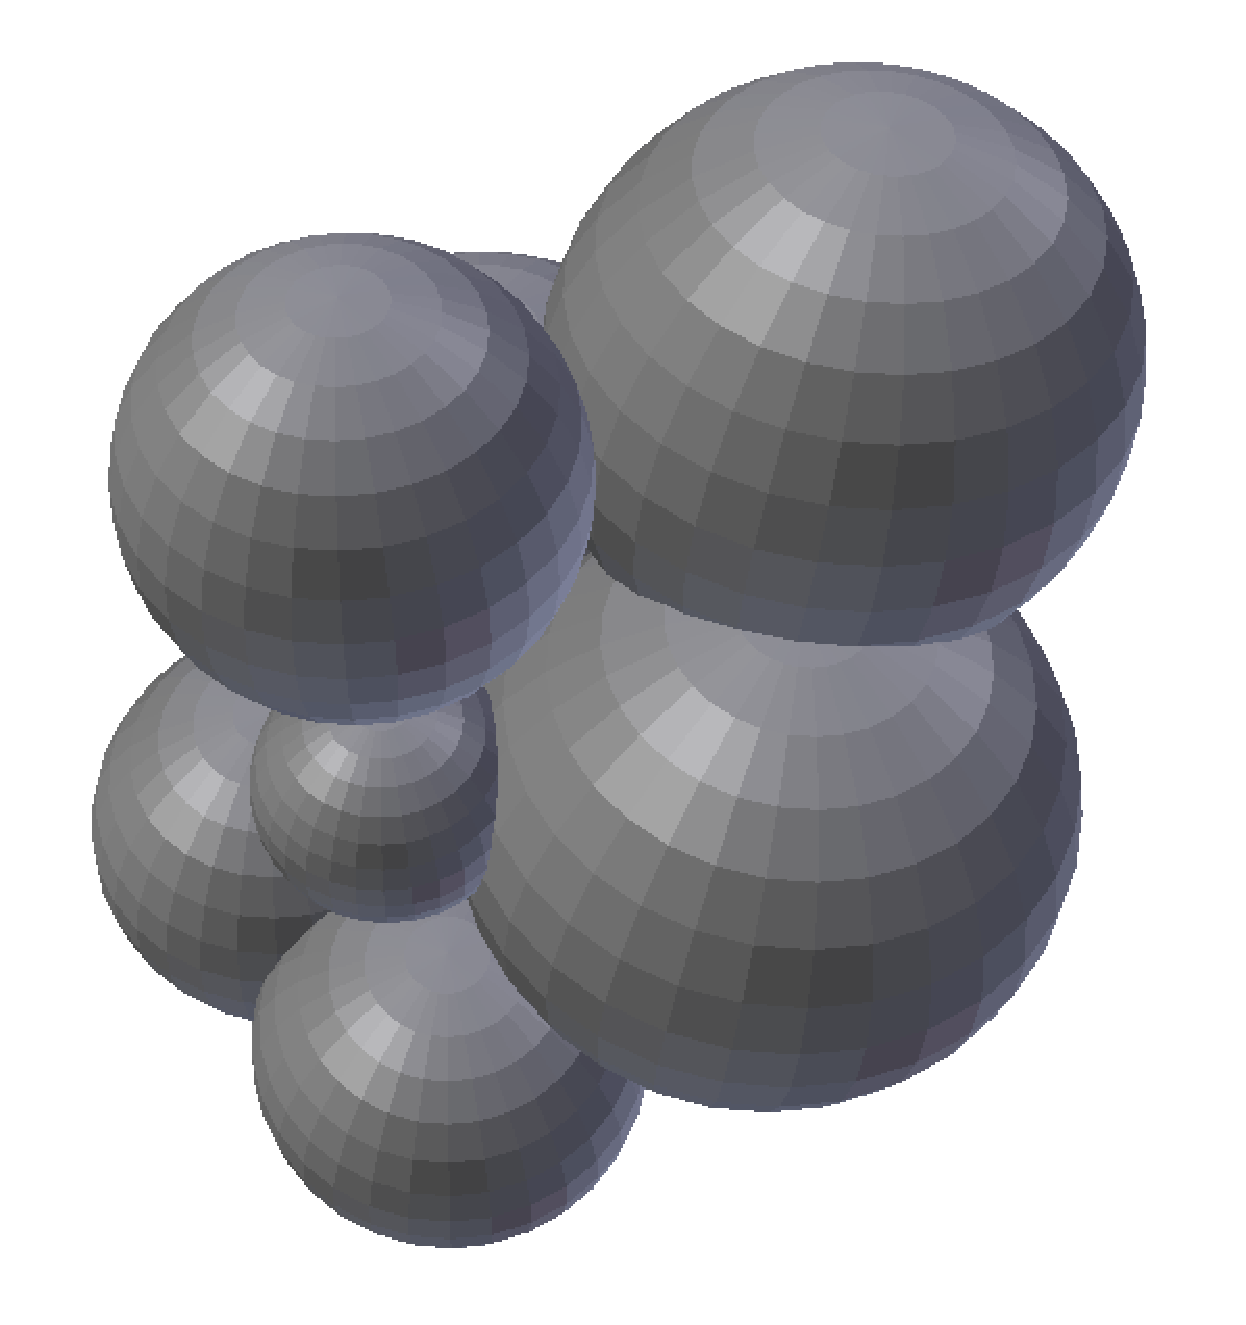
\includegraphics[width=0.45\linewidth]{figures/clunk}
		% \begin{verbatim}
		%         rand(objs)
		% \end{verbatim}
	\end{minipage}%
	\begin{minipage}[t]{5cm}
		\centering
		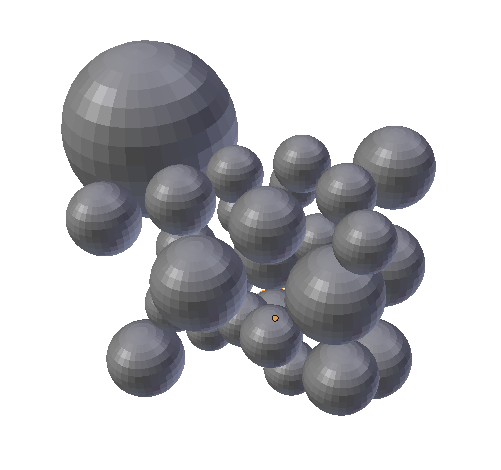
\includegraphics[width=0.45\linewidth]{figures/render}
		% \begin{verbatim}
		% pred = nointersect(objs)
		% rand(scene, pred)
		% \end{verbatim}
	\end{minipage}%
	% \begin{minipage}[t]{5cm}
	% \centering
	% 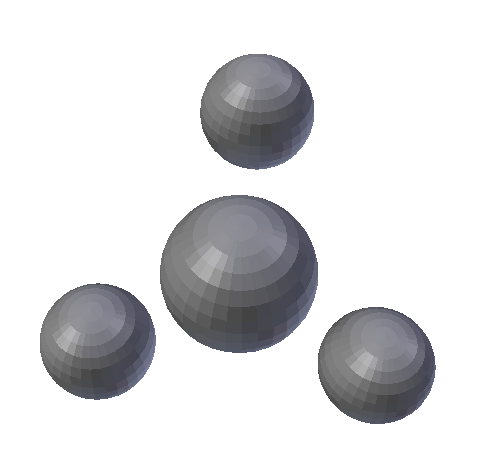
\includegraphics[width=0.5\linewidth]{figures/equi}
	% $$
	% x = 3
	% $$
	% % \begin{verbatim}
	% % pred = equidistant(objs)
	% % rand(scene, pred)
	% % \end{verbatim}
	% \end{minipage}
	\caption{A weak prior (left) does not respect rigid body constraints on objects, whereas (center) is conditioned on the predicate that objects don't intersect.  (right) objects are conditioned on being equidistant, resulting in a tetrahdral arrangement}
	\label{fig:nointersect}
\end{figure}


\paragraph{Random Variables.} Probability models lie on top of probability
spaces. A probability space is a measure space $(\Omega, {\cal H}, {\cal P})$,
where ${\cal H}$ is a sigma algebra and ${\cal P}(\Omega) = 1$ \citep{ccinlar2011probability}. Random variables are
functions from the space $\Omega$ to a realization space ${\cal X}$. As a concrete
example the space $\Omega$ can be thought of as a hypercube, with ${\cal P}$ being
uniform over that hypercube. To build a normal random variable, we need a function
that maps from $\Omega \to \mathbb{R}$. If the underlying probability space is uniform, then
this function is the inverse cumulative distribution function of the normal.

A \emph{model} $\cM$ is a collection of random variables along with a probability space.
% To fully specify a model, we need both the measure space and the
% collection of random variables on which it acts.

\paragraph{Conditioning}

Conditioning a model creates a new model.
As an example consider a model $\cM$ with two
random variables $X_1$ and $X_2$ that both take real values. Conditioning
$\cM$ on $X_1 = 1$, defines a new model $\cM_{|A}$ based on limiting the measure space
$\Omega$ to the set $A = \{ \omega : X_1(\omega) = 1\}$.
The new model is defined on a new probability space
\begin{align}
	(\Omega \cap A, \{A \cap B, B \in {\cal H} \}, {\cal P} / {\cal P}(A))
\end{align}
with the same random variables $X_1$ and $X_2$.
Sampling from $\cM_{|A}$ produces
samples only where $X_1 = 1$

More generally, conditioning on any predicate $Y(\omega) = \lk(X_1(\omega), \dots, X_n(\omega))$
defines a new model defined exactly as above, where $A = \{\omega : \lk(X_1(\omega), \dots, X_n(\omega)) = 1\}$.
% This predicate may include a comparisonsuch as $X_i < X_j$, restrict deterministic function of variables in in the model such as $\exp(X_i) = 2$, or be a Boolean combination such as $(X_i < X_j) \lor \neg(\exp(X_i) = 2)$.
Sampling from $\cM_{|A}$ generates $(x_1, ..., x_n)$ where $\lk$ is true.

The general construction of new models might require conditioning
on sets of measure zero. This process can be made rigorous
via disintegration \citep{chang1997conditioning}. Disintegration can
be thought of as the reversal of building joint distributions through
product measure constructions.


% When building models with prior beliefs via conditioning, we would like
% the property that given an infinite collection of observations, the 
% posterior predictive distribution converges to true sampling distribution.
% To study this, consider a model with two random variables that are independent,
% $X_1$ is a function of $\omega_1$ and $X_2$ is a function of $\omega_2$. Suppose
% that the true sampling distribution has $X_1$ and $X_2$ positively correlated.
% For the prior beliefs to support positive correlations, we 
% could condition on a prior belief that $X_1$ and $X_2$ are close. However
% if the form of the closeness isn't controlled by a random variable, observing
% an arbitrary amount of data from the true distribution will not change
% the dependence between $X_1$ and $X_2$ in the model. 
% \begin{align*}
% X_j^*(\omega^*) = \sigma(f_\Beta(X_{j, 1}, ..., X_{j, n})) > b, \\
% \end{align*}
% Conditioning on $X_j^*$ produces a new set of models that have 
% dependence between . Knowledge is encoded in the prior distribution
% on $\Beta$. If $f_\Beta$ has priors over the true dependence between
% $X_{., 1},...,X_{., m}$, then this new model family will converge
% to the true underlying distribution.

% rr: TODO the above can me made into a proof

% \subsection{Bayesianism vs. Bayesian Computation}
% The way we 


% \section{Higher Order Random Variables}
% People often entertain beliefs about probability statements. For instance most people accept 
% trust expert-given odds that a particular sports team will win a tournament, 
% or politician will win an election, more than the odds of those given by non-experts.
% The apparent failure of probabilistic expressions to distinguish 
% between these cases led to alternative formalisms of uncertainty \citet{Shampher}, 
% but within the probabilistic framework both \citet{Pearl} and \citet{Hyberg} demonstrated 
% that such higher order distributions were induced from the original model, no new machinery was needed.

% As a concrete example of this, suppose we have a stochastic 
% dynamical system model of human blood glucose 
% controlled by some 
% parameters $\Theta$ with a prior. A priori we know that the average blood pressure 
% in a person lives in a physically plausible range $40-400$. A way to
% encode this would be to change the prior on the parameters $p(\Theta)$ 
% to so that any sample from that prior yields has average in the physically
% plausible range. This can be challenging because it requires a detailed
% understanding of the stochastic dynamical system. 

% Alternatively, we could try to take the conditioning approach from the
% previous section. But conditioning in the previous section required explicitly
% defined random variables, and while the average glucose is a random variable
% because the parameter $\Theta$ is random, it is not an explicit random variable.
% The scenario requires the ability to both define and condition on 
% probability distributions over either random variables or properties of 
% random variables (e.g. expectations).
% In this section we introduce the random conditional 
% distribution ($\randcond$) to support this task.

% \paragraph{The Random Conditional Distribution.}
% The random conditional distribution of $X$ given $\Theta$ -- which we denote $\rcd(X, \Theta)$ or $\rcdxy{X}{\Theta}$ -- is a random distribution: a random variable which takes values in the domain of random variables.
% Informally, $\rcdxy{X}{\Theta}$ is a function of $\omega$ that returns functions of $\omega$
% of the same type as $X$. Formally, $\rcd$ is a distribution over conditional random variables:

% % The primary mechanism for conditioning is $\cond$, which constructs conditional random variables:
% % \begin{definition}
% % Let $X:\Omega \to T$ be a random variable, $Y$ an indicator function, and $\conds{X}{Y}: \Omega_{|Y} \to T$ be a conditional random variable defined as: $X_{|Y}(\omega) = X(\omega)$.
% % $X_{|Y}$ is defined on a conditioned probability space $(\Omega, \Sigma, \mu_{|Y})$ where $\mu_{|Y}$ is a conditional measure: $
% % \mu_{|Y}(A) = \mu(A \cup Y^{-1}(\{1\})) / \mu(Y^{-1}(\{1\})$.
% % % That is, $\cond: (\Omega \to T) \times (\Omega \to \{0, 1\}) \to (\Omega \to T)$ is a operator that restricts the domain of $X$ to those inputs consistent with $Y$.
% % \end{definition}


% \begin{definition}The random conditional distribution of a random variable $X: \Omega \to T_1$ given $\Theta: \Omega \to T_2$ is a random variable $\rcdxy{X}{\Theta}: \Omega \to (\Omega \to T_1)$, defined as:
% \begin{equation}\label{eq:rcd}
% (\rcdxy{X}{\Theta})(\omega) = [\conds{X}{\Theta = \Theta(\omega)}]
% \end{equation}
% \end{definition}
% For example if $\Theta = \bern(0.4)$ and $X = \normal(\Theta, 1)$, then $\rcdxy{X}{\Theta}$ is a random distribution 
% whose domain comprises of two normal distributions $X_1 = \conds{\normal(\Theta, 1)}{\Theta = 1}$ and $X_2$.
% The probabilities of $X_1$ and $X_2$ with respect $\rcdxy{X}{\Theta}$ are determined by the prior probabilities of the different outcomes of $\Theta$: $P((\rcdxy{X}{\Theta}) = X_1) = 0.4$ and $P((\rcdxy{X}{\Theta}) = X_2) = 0.6$.

% A random conditional distribution is most useful in combination with other functions.
% Expectation is perhaps the most important example, which when composed with $\rcd$ produces conditional expectation.
% Restricting to real valued variables, expectation $E$ is a functional that maps a random variable to a real value
% (($\Omega \to \mathbb{R}) \to \mathbb{R}$).
% When $X$ is a real valued random variable, $\rcdxy{X}{\Theta}$ is not real valued, and hence not a valid argument to $E$.

% However, just as arithmetic operations such as $+$ and $-$ extend from the domain of numbers to the domain of random variable (pointwise $X + Y = \omega \mapsto X(\omega) + Y(\omega)$), $E$ extends from the domain of random variables to the domain of random variables over random variables in precisely the same way.
% % Since random variables are themselves functions, $E$ is an operator, functional or more generally a higher-order function.  
% % As described in section X a function with domain $T$ can be lifted to a functional of $T$-valued random variables.
% % $T$ is purposefully left abstract, because in addition to lifting functions defined on the reals etc, we can lift functions defined on random variables.
% % Expectation is a cannonical example of a random variable valued function, with type $E : (\Omega \to \mathbb{R}) \to \mathbb{R}$.
% That is, $\ee$ has a lifted counterpart $\lifted{\ee} = \lift(\ee)$ with type $\lifted{\ee} : (\Omega \to (\Omega \to \mathbb{R})) \to (\Omega \to \mathbb{R})$, which maps a distribution over real valued random variables to a distribution over real values (expectations).
% % $$
% % \lifted{\ee}(X)(\omega) = \mean{X(\omega)}
% % $$
% The operator $\rcd$ composed with $\ee$ constructs conditional expectation (with respect to a random variable $\Theta$):
% \begin{equation}
% \lmean{\rcdxy{X}{\Theta}} = \lmean{\omega \mapsto \conds{X}{\Theta = \Theta(\omega)}} 
%                     = \omega \mapsto \mean{\conds{X}{\Theta = \Theta(\omega)}}\\
% \end{equation}
% The final term $\omega \mapsto \mean{\conds{X}{\Theta = \Theta(\omega)}}$ matches the definition of
% conditional expectation
% with respect to a random variable $\mean{(X\mid \sigma (Y))(\omega)} = \mean{X \mid Y = Y(\omega))}$.
% That is the conditional expectation is a random variable with randomness provided by the conditioning set.

% Returning to the blood glucose example, we can build a model that respects the valid range
% of average blood glucose by taking the original model creating the conditional expected
% value of glucose $G$ with $\rcd$ and expectation of $\rcd$, then constructing a new model
% by conditioning the original on $G$ being in the physiologically possible range.

% \paragraph{Completeness.}Nested uses of $\rcd$ lead to a completeness result. State informally: 
% by repeatedly applying $\rcd$, any random function or functional in the original model
% can be constructed. Then by using conditioning to create new models from the previous 
% section, we can alter existing models to respect predicates on any random quantity in
% the model even if the random quantity is not an explicit random variable.
% % RR: TODO: The above could be a theorem


\section{Predicate Exchange}

% Predicate exchange is /a procedure to sample from a model conditioned on a predicate.
% To condition a model on a predicate we develop \emph{predicate exchange}, a likelihood-free inference procedure. 
Given a model (a collection of random variables)  $\vect{X} = (X_1, X_2, \dots, X_n)$ and a predicate $\lk$ which maps a model realization  $\vect{x} = (x_1, x_2, \dots, x_n)$ to 0 or 1, predicate exchange samples from the posterior distribution of $\vect{X}$ conditioned on $\ell$ through two steps:
\begin{enumerate}
\item \textbf{Predicate Relaxation} constructs a soft predicate $\soft{\lk}$ from $\lk$. $\soft{\lk}$ takes values in a continuous Boolean algebra: the unit interval $[0, 1]$ with continuous logical connectives $\soft{\land}$, $\soft{\lor}$ and $\neg$.
$\soft{\lk}$ is 1 iff $\lk$ is 1, but otherwise takes nonzero values denoting the degree to which $\lk$ is satisfied.
% The relaxation is parameterized by a temperature.
% Predicate relaxation allows us to apply likelihood based MCMC inference procedures.
\item  \textbf{Replica Exchange} is a Markov Chain Monte Carlo procedure that simulates several replicas of $\soft{\lk}$ in parallel. 
\end{enumerate}

In this section we formalize the construction of $\soft{\lk}$ from $\lk$, and sampling from models conditioned on $\soft{\lk}$.

\subsection{Predicate Relaxation}\label{predexchange}

Our objective is to construct a soft predicate $\soft{\lk}$ that introduces approximations into $\lk$ to make inference more tractable.
Informally, these approximations mean that while conditioning on $\lk$ eliminates a set of possible values, soft conditioning on $\soft{\lk}$ only makes them less likely.
% Formally, $\soft{Y}$ approximates
% the sense that \todo{IN WHICH WAY?}when viewed as a likelihood function on model parameters, $\soft{\lk}$ has a broader support, assigning nonzero weights to parameter values which have zero weight under $\lk$.

There are three desiderata which govern this approximation.
$\soft{\lk}$ should have a temperature parameter $\alpha$ that controls the fidelity of the approximation. In particular, $\soft{\lk}$ should (i) converge to $\lk$ as $\alpha \to 0$, (ii) converge to 1 as $\alpha \to \infty$, and (iii) be consistent with $\lk$ on 1, i.e., $\lk(\vect{x}) = 1$ iff $\softv{\lk}(\vect{x}) = 1$ at all temperatures.  
Formally:

% The family of approximations of the predicate $Y$ is parameterized through a temperature $\alpha$ that controls the smoothness of the approximation. In particular, $\soft{\lk}$ with $\alpha \to 0$ converges to $Y$ itself while increasing values of $\alpha$ yield smoother approximations eventually giving a flat surface when $\alpha \to \infty$. Moreover, the set of conditional samples $C(Y) = \{ \omega \in \Omega \text{ } | \text{ } Y(\omega) = 1 \}$ are assigned a value of $1$ in $\soft{\lk}$ for all temperatures. 

% To construct a $\soft{\lk}$ with such properties, we let $Y$ be the following predicate $a=b$ for standard Gaussians $a, b \sim \mathcal{N}(0, 1)$. We choose a distance
% $\rho(a, b)$ to indicate how close our sample is to $C(Y)$. To meet the desiderata
% of having $C(Y)$ be $1$ over the constraint set and to ensure the constraint becomes
% smoother with large $\alpha$, we use a function $k : [0, \infty] \to [0, 1]$ parameterized by $\alpha$ to wrap the distance $\rho(a, b)$. A simple choice for such a function is $k(d; \alpha) = e^{-d / \alpha}$ that provides the desired properties to $\soft{\lk}$ (see Appendix). The formal definition of $\soft{\lk}$ is as follows.

\begin{definition}
$\softv{\lk} : \xp \to [0, 1]$ parameterized by $\alpha \in [0, \infty)$ is a relaxation of $\lk: \xp \to \{0, 1\}$ if for all $\vect{x} \in \xp$:
\begin{enumerate}[label=(\roman*)]
	\label{def:temp}
	\item $\lim_{\alpha \to 0}\softv{\lk}(\vect{x}; \alpha) = \lk(\vect{x})$.
	\item $\lim_{\alpha \to \infty}\softv{\lk}(\vect{x}; \alpha) = 1$.
  \item for all $\alpha < \infty$, $\softv{\lk}(\vect{x}; \alpha) = 1$ iff $\lk(\vect{x}) = 1$.
\end{enumerate}
\end{definition}

\todo{Explain motivate each of these desiderata}

\paragraph{Distance Based Satisfiability}
To construct $\soft{\lk}$ we assume $\xp$ has a metric, and define $\softv{\lk}(\vect{x})$ -- the degree to which $\vect{x}$ satisfies $\lk$ -- as the \emph{distance} from $\vect{x}$ to an element in $\xp$ that satisfies $\ell$.
Concretely, the \emph{tightest} relaxation of $\ell$ is:

\begin{definition}
Let $\rho$ be a metric on $\xp$, $k_\alpha$ be a relaxation kernel (described below) which bounds distances to $[0, 1]$, and $A = \{\vect{x} \mid \lk(\vect{x}) = 1\}$ be the \emph{satisfying set}.
The predicate $\soft{\lk}_{\inf}(\vect{x})$ is a tightest relaxation of $\ell$ and defined as:
\begin{equation}
\soft{\lk}_{\inf}(\vect{x}) = k_\alpha(\rho(\vect{x}, A))
\end{equation}
The distance $\rho(\vect{x}, A) = \inf \left\{\rho(\vect{x}, a) \mid a \in A\right\}$ is the smallest distance between $\vect{x}$ and any element of $A$.
% As shown in the Section \ref{implement}, $\soft{\lk}_{\inf}$ can be difficult to compute.
\end{definition}

% \paragraph{Product Metrics}The metric $\rho$ is parameterized by the type of input.
% For canonical spaces such as $\mathbb{R}$ and $\mathbb{N}$ we default to the Euclidean distance. 
% We can construct $\rho$ automatically for composite elements $x, y \in \mathbb{T}_1 \times \cdots \times \mathbb{T}_n$ of product types, by taking the mean of distances of components: $\rho(x, y) = (1/n)\sum^n_{i=1}\rho(x_i, y_i)$.

% $$
% d_{p}((x_{1},\ldots ,x_{n}),(y_{1},\ldots ,y_{n}))=\|\left(d_{X_{1}}(x_{1},y_{1}),\ldots ,d_{X_{n}}(x_{n},y_{n})\right)\|_{p}}
% $$

\paragraph{Relaxation Kernels} A relaxation kernel $k_\alpha$ bounds distances from $\mathbb{R}$ to the unit interval, and is paramterized by temperature $\alpha$.
% For example if $x$ and $y$ are real values, then $x \soft{=} y$ is defined as $k_\alpha(\rho(x, y))$ where $\rho$ is a distance function and $k_\alpha$ is a relaxation kernel paramterized by temperature $\alpha$.
% A relaxation kernel maps distances to values in $[0, 1]$, and ensures that $\soft{\lk}$ adheres to the outlined criteria.
Relaxation kernels are responsible for ensuring consistency with the relaxation criteria.
We restrict our attention to the squared exponential kernel:
\begin{equation}
k_{\alpha}(r) = \exp\left(-\frac{r^2}{\alpha}\right)
\end{equation}




  % \begin{center}
  % \begin{tabular}{ c |  c | c }
  %   \hline		
  %   $x \soft{=} y$ & $x \soft{>} y$ & $x \soft{<} y$  \\
  %   $k_\alpha(\rho(x, y))$ & $k_\alpha(\rho(x, [y, \infty]))$ & $k_\alpha(\rho(x, [-\infty, y]))$ \\
  %   \hline  
  % \end{tabular}
  % \end{center}



\paragraph{Composition of Soft Primitives} We construct $\soft{\lk}$ from $\lk$ compositionally, by substituting primitive predicates (equality, inequalities and logical operators) with soft counterparts.
For instance the predicate $(x > y) \lor \neg(x^2 = 2)$ is transformed into $(x \soft{>} y) \soft{\lor} \softv{\neg}(x^2 \soft{=} 2)$.
In general, we use $\soft{p}$ to denote a relaxation of a predicate $p$.
% \begin{figure}[H]\label{softpreds}
%   \begin{align*}
% x \soft{=} y &= k_\alpha(\rho(x, y))\\
% x \soft{>} y &= k_\alpha(\rho(x, [y, \infty]))\\
% % x \soft{<} y &= k_\alpha(\rho(x, [-\infty, y]))\\
% x \soft{<} y &= k_\alpha(\rho(y, [-\infty, x]))\\
% a \soft{\land} b &= \max(a, b)\\
% a \soft{\lor} b &= \min(a, b)
% \end{align*}
% \caption{Soft Primitive Predicates}
% \end{figure}

Soft equality is straightforward: $x \soft{=} y$ is defined as $k_\alpha(\rho(x, y))$.
A soft inequality such as $x \soft{>} y$ is a function of the amount by which $x$ must be increased (or $y$ decreased) until $x > y$ is true.
This is the distance between $x$ and the interval $[y, \infty]$, where the distance between a point and any interval $[a, b]$ is the smallest distance between $x$ and any element in $[a, b]$, and therefore 0 if $x \in [a, b]$:
\begin{equation}
\rho(x, [a, b]) =
\begin{cases}
  a - x & \text{ if } x < a\\
  x - b & \text{ if } x > b\\
  0              & \text{otherwise}
\end{cases}
\end{equation}
Soft conjunction $\soft{\land}$ and disjunction $\soft{\lor}$ take the $\min$ and $\max$ respectively, which is standard.
Soft negation, on the other hand, introduces complications.
In continuous logics \cite{kimmig2012short}, the negation of $a \in [0, 1]$ is $1 - a$.
However, as shown in Figure \ref{negationimg} (b), this violates criteria (iii) of predicate relaxation; there are values which satisfy the hard predicate $\neg(x > 0)$ which do take a value of 1 in $1 - (x \soft{>} 0)$.
Figure \ref{negationimg} illustrates this issue.


\begin{figure}
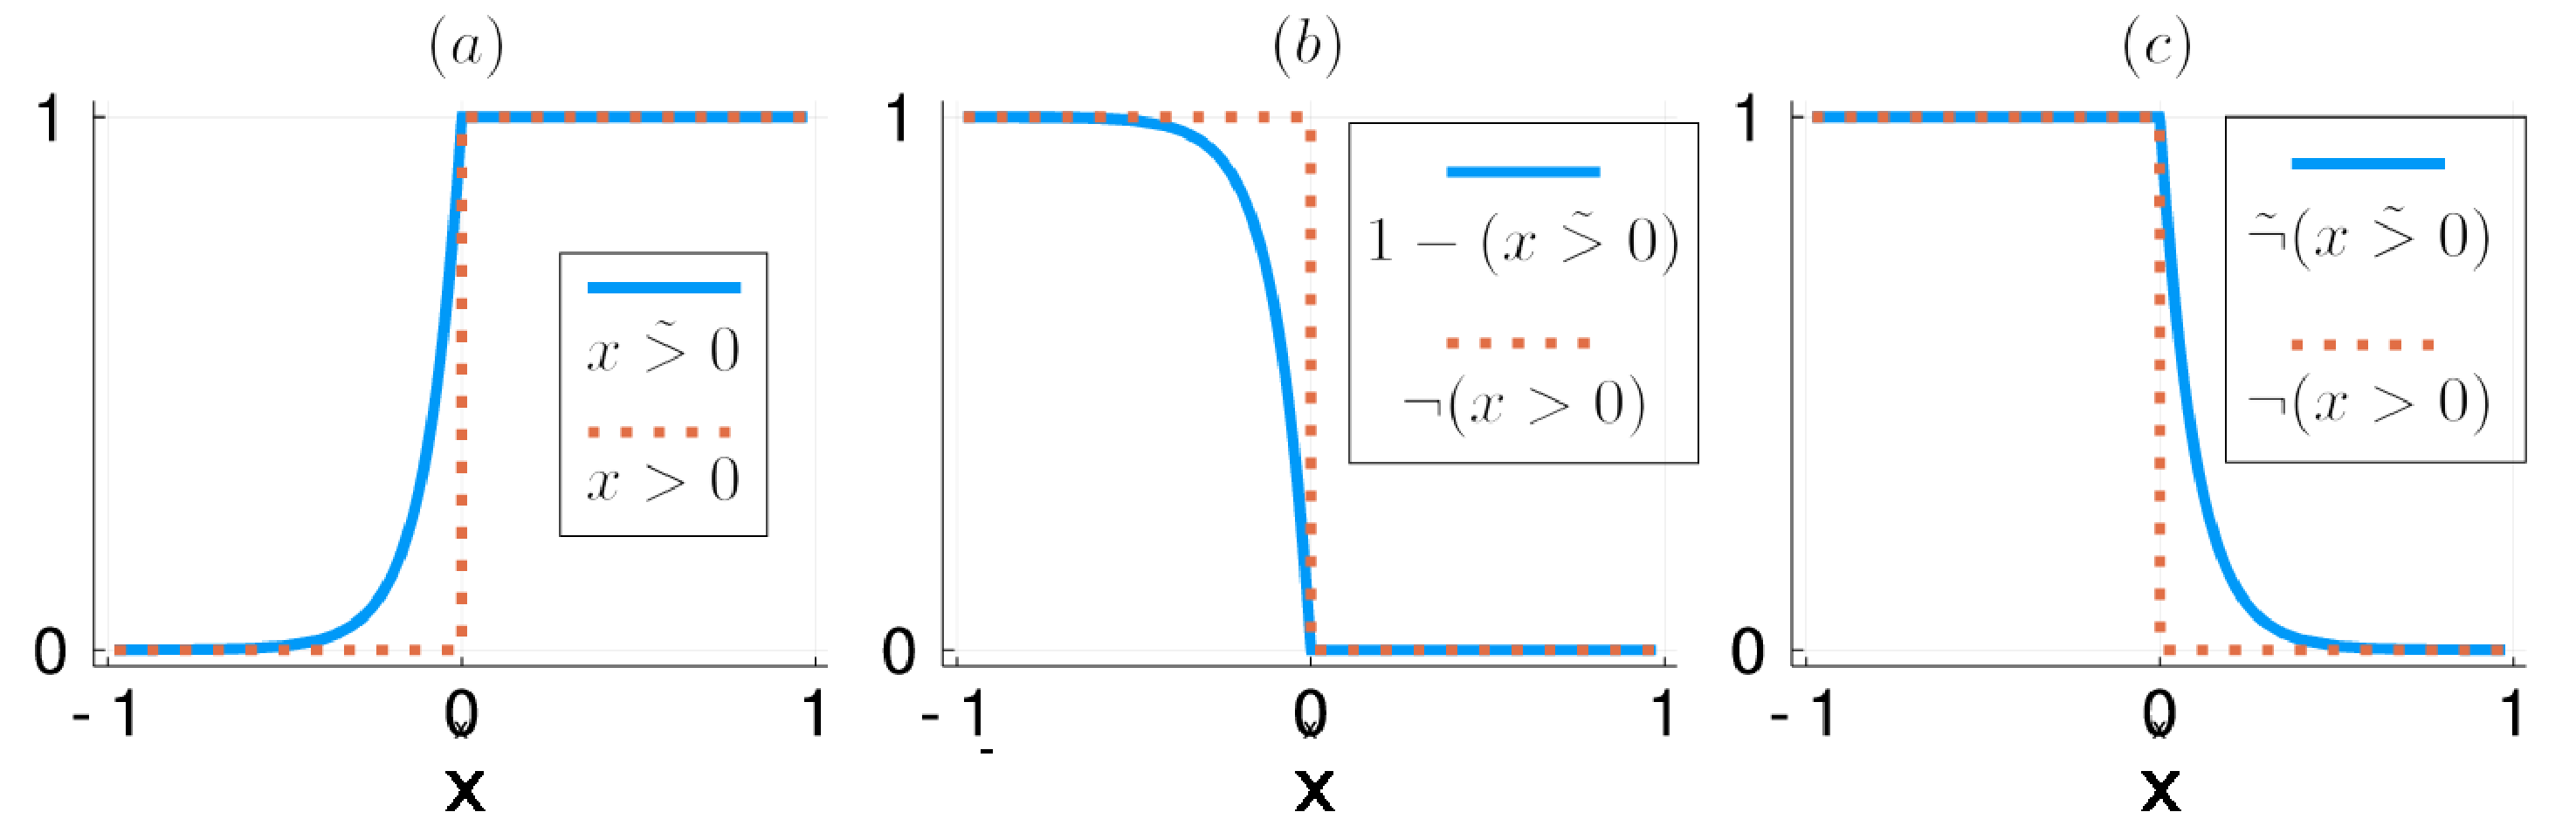
\includegraphics[width=\linewidth]{negation.eps}
\caption{Negation: soft (blue) and hard (red, dashed) predicates as a function of $x$.  Left: $x \soft{>} y$ approximates $x > y$. Middle:  Standard approach to continuous negation $(1-a)$ violates relaxation criteria. Right: Desired outcome of soft negation of $x \soft{>} y$.}\label{negationimg}
\end{figure}


The problem of negation arises because $\soft{\lk}$ is consistent with $\lk$ at 1 but not at 0.
In other words, $\soft{\lk}$ is a one-sided approximation.
To resolve this, \emph{two-sided} soft primitives yield a pair $(a_0, a_1)$ where $a_0, a_0 \in [0, 1]$.
$a_1$ preserves consistency with $\lk$ on $1$, just as before, while $a_0$ preserves consistency with $\neg \lk$ on $1$.
For example if $x \dsoft{>} 0$ returns $(a_0, a_1)$, then as a function of $x$, $a_0$ and $a_1$ correspond to Figure \ref{negationimg} (a) and (c) respectively.
Soft negation then simply swaps the elements of $(a_0, a_1)$ to yield $(a_1, a_0)$.

A complete two-sided soft logic is shown in Figure \ref{softw}.
When we condition on a model, however, \rework{stil lconcerned is not informative} we are still concerned on with the true side, i.e. $a_1$ in the pair $(a_0, a_1)$.

% \begin{definition}
% The function $\softv{Y} : \Omega \to [0, 1]^2$ parameterized by $\alpha \in [0, \infty)$ is a two-sided relaxation of a $Y: \Omega \to \{0, 1\}$ if:
% \begin{enumerate}[label=(\roman*)]
% 	\label{def:temp}
% 	\item For all $\omega \in \Omega$, $\lim_{\alpha \to 0}\softv{Y}(\omega; \alpha) = (\neg Y(\omega), Y(\omega))$.
% 	\item For all $\omega \in \Omega$, $\lim_{\alpha \to \infty}\softv{Y}(\omega; \alpha) = (0, 1)$.

%     \item For all $\alpha$, $\softv{Y}(\omega; \alpha) = 1$ iff $Y(\omega) = 1$.
%     \item The entropy $H(\softv{Y}(\omega; \alpha))$ (which characterizes the fidelity of the approximation ) is an increasing function of $\alpha$.\footnote
%     {By compactness, it is integrable for all $\alpha$, when $\Omega$ has finite dimension}
% \end{enumerate}
% \end{definition}


\begin{figure}
\begin{align*}
x \dsoft{=} y &= (\text{if } x = y  \text{ then } \exp(-1/\alpha) \text{ else } 1, k_\alpha(\rho(x, y)))\\
x \dsoft{>} y &= (k_\alpha(\rho(x, [-\infty, y])), k_\alpha(\rho(x, [y, \infty])))\\
x \dsoft{<} y &= (k_\alpha(\rho(y, [x, \infty])), k_\alpha(\rho(y, [-\infty, x])))\\
(a_0, a_1) \dsoft{\land} (b_0, b_1) &= (\min(a_0, b_0), \min(a_1, b_1))\\
(a_0, a_1) \dsoft{\lor} (b_0, b_1) &= (\max(a_0, b_0), \max(a_1, b_1))\\
\softv{\neg}(a_0, a_1) &= (a_1, a_0)
\end{align*}
\caption{Two-sided soft primitive predicates}
\label{softw}
\end{figure}

% \begin{center}
% \begin{tabular}{ l | c | r }
%   % \hline		
%   $(a_0, a_1) \soft{\land} (b_0, b_1)$ & $(a_0, a_1) \soft{\lor} (b_0, b_1)$ & $\neg(a_0, a_1)$ \\
%   $(a_0, a_1) \soft{\land} (b_0, b_1)$ & $(a_0, a_1) \soft{\lor} (b_0, b_1)$ & $\neg(a_0, a_1)$ \\
%   % \hline  
% \end{tabular}
% \end{center}
\begin{proposition}Relaxation criteria are preserved under composition.
Let $a$ and $b$ be predicates, and $\circ$ denote a binary logical operator.  If $\softv{a}, \softv{b}$ and $\soft{\circ}$ are respective valid relaxations.  Then $\softv{a} \soft{\circ} \softv{b}$ is a relaxation of $a \circ b$.
\end{proposition}
% \emph{proof} Prove it.



\subsection{Approximate Markov Chain Monte Carlo}
A soft predicate can serve as an approximate likelihood, and as a result is amenable to likelihood based inference methods such as Markov Chain Monte Carlo.
MCMC algorithms require a function $f$ that is proportional to the the target density.
In Bayesian inference this is the posterior, dictated by Bayes' theorem as the product of the likelihood and the prior.
Approximate inference using soft predicates takes a similar form.

\begin{definition}
Let $\vect{X} = (X_1, \dots, X_n)$ be a model, $\lk$ be a predicate that conditions $\vect{X}$, and  $\vect{x}$ be a relaxation of $\vect{X}$.
Assuming a prior density $p$, the approximate posterior $f$ is the product:
\begin{equation}\label{fpm}
f(\vect{x}) = p(\vect{x}) \; \cdot \soft{\lk}(\vect{x})
  \end{equation}
\end{definition}
$\soft{\lk}$ down weights parameter values which violate $\lk$ by the degree to which they violate it. 
This is modulated by the temperature $\alpha$ used in the  relaxation kernels which constitute $\soft{\lk}$.
At maximum temperature $\soft{\lk}$ has no effect, and the approximate posterior $f$ is equal to the prior $p$.
At zero temperature, $f$ recovers the true posterior since parameter values which violate the condition are given zero weight.

For illustration, let $\vect{X} = (\mu, X)$ be a model where $\mu = \beta(3, 4)$ and $X = \mathcal{N}(\mu, 1)$.
If conditioned on $X = 0.5$, the approximate posterior is shown at different temperatures in Figure \ref{temppost} and defined as:
\begin{equation}\label{approxposterior}
f_\alpha(\mu, x) = \beta_{0,1}(\mu) \cdot \mathcal{N}_{\mu,1}(x) \cdot k_\alpha(\rho(x, 0.5)) 
\end{equation}

%  q
The temperature parameter trades off between tractability of inference and the fidelity of the approximation.
If the temperature is too high and $\soft{\lk}$ will diverge too greatly from $\lk$. If it is too low, convergence will be slow.

\paragraph{Balancing Different Constraints}
At a fixed, nonzero temperature, the scales of variables affects their influence on
the conditional distribution.
For instance, consider two uniformly distributed random variables $x \sim \unif(-1, 1)$ and $y \sim \unif(-10, 10)$,
and predicates $p_x = x \soft{=} 0$ and $p_y = y \soft{=} 0$.
The expectation of a soft predicate quantifies the degree to which it is true (see Section \ref{simmodels}).
The prior expectation of $p_x$ is significantly larger than that of $p_y$.
because values far from the 0 are more likely under $y$.

This disparity persists if model is conditioned.
Figure \ref{scaling} shows samples from the model conditioned on $p_x \soft{\lor} p_y$, and a disparity in the histograms of $p_x$ and $p_y$.
The disparity decreases with decreasing temperature, and disappears at zero.
Still, it is undesirable in practice because it means that the approximation error is distributed unevenly.

% For example consider two pairs of variables, where
% the first pair is ten times larger than the second.
% Conditioning on a greater than constraint on both
% pairs of variables is well defined. However,
% a softening of both constraints would have 
% a much larger change in the energy function over
% a standard deviation change in pairs of variables.
To mitigate this issue, we minimize discrepancies between sample averages of constraints
Consider the case of two 
soft predicates $k_1$ and $k_2$. We introduce a weight for all but the first constraint.
In this case $k_2$ in the soft predicate is replaced
by $\gamma_2 k_2$. The weight $\gamma_2$ should
ensure that $\gamma_2 k_2$ has the same
magnitude effect as $k_1$ on the energy
function:
\begin{align*}
E_{p_{\alpha, \gamma_2}}[k_1] = E_{p_{\alpha, \gamma_2}}[\gamma_2 k_2] 
\end{align*}
% Does such a gamma_2 always exist? Maybe rewrite it as
% an optimization problem over gamma to enforce a solution?
In practice, we set $\gamma_2$ using an exponential moving
average of the $k_1$ values over the $k_2$ values.
Figure \ref{scaling} visualizes the problem of unbalanced constraints, as well as corrections to $\gamma$.


\begin{figure}
  \centering
  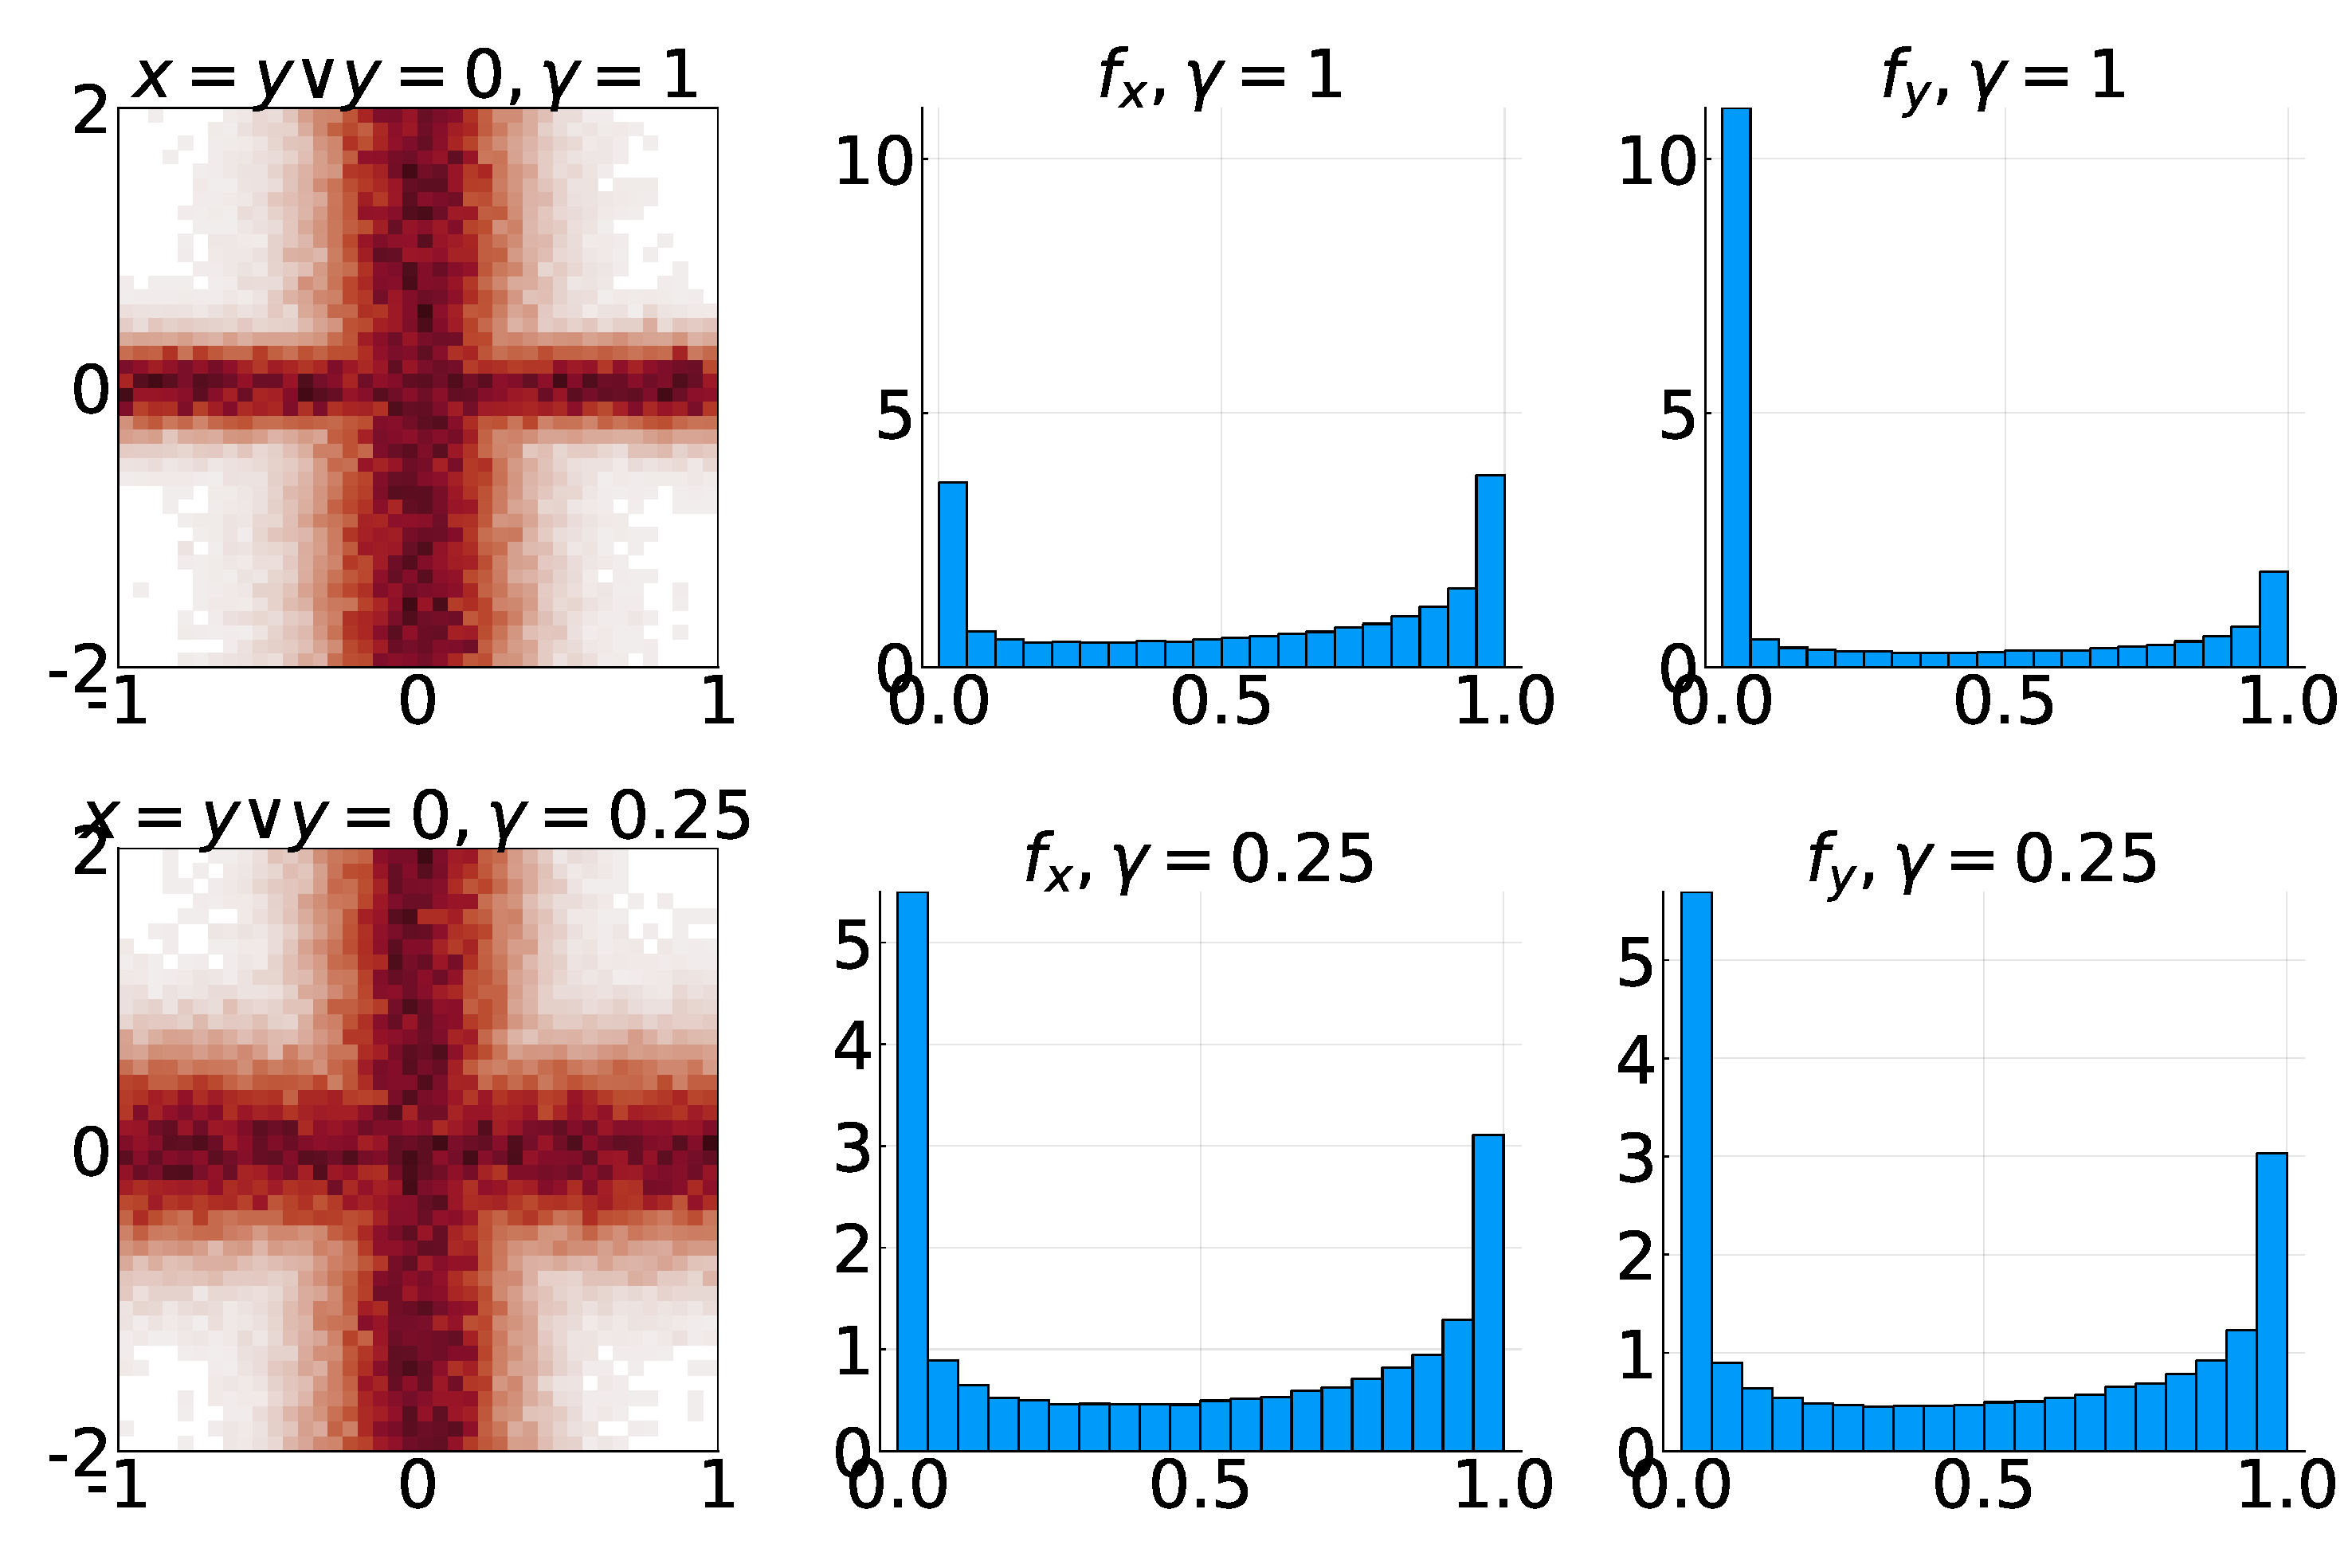
\includegraphics[width=0.9\linewidth]{scaling.pdf}
  \caption{Scaling Properties.}\label{scaling}
  \end{figure}

  
\subsection{Replica Exchange}\label{replicaexchange}
Replica exchange \citep{swendsen1986replica} simulates $M$ replicas of a model at different temperatures, and uses a Metropolis-Hastings update to  periodically swap the temperatures of chains.
Let $f_{\alpha_i}$ denote the approximate posterior function at temperature $\alpha_i$, then two independent parallel chains simulating targets $f_{\alpha_1}(x)$, $f_{\alpha_2}(y)$  follow a joint target $f_{\alpha_1, \alpha_2}(x,y) = f_{\alpha_1}(x)f_{\alpha_2}(y)$.
Replica exchange swaps states between the chains while preserving the joint target.
Swapping states is equivalent to swapping predicates, which motivates the name ``predicate exchange''.
Concretely, replica exchange proposes a swap from $(x, y)$ to $(y, x)$, and accepts it with probability $\min(1, A)$, where:
\begin{equation}
A =  \frac{f_{\alpha_1, \alpha_2}(y,x)}{f_{\alpha_1, \alpha_2}(x,y)} = \frac{f_{\alpha_1}(y)f_{\alpha_2}(x)}{f_{\alpha_1}(x)f_{\alpha_2}(y)}
\end{equation}

We modify standard replica exchange in two ways: (i) for exact inference, states which violate the constraint are rejected, and (ii)
unlike conventional replica exchange which draws samples only from the zero-temperature chain, we accept states from any chain so long as $f_{\alpha_i}(x) = 1$.

Replica exchange has a number of hyper-parameters: the number of parallel chains, the corresponding temperatures, the swapping schedule.
Several good practices are outlined in \cite{earl2005parallel}.  In practice, we logarithmically space $\alpha$ between a lower and upper bound (e.g., $\log_{10}(\alpha_1) = 5$ to $\log_{10}(\alpha_M) = -5$), and swap states of chains that are adjacent in temperature ($\alpha_1$ with $\alpha_2$, $\alpha_2$ with $\alpha_3$, etc) periodically.

% \paragraph{Unsatisfiability}Predicate exchange is unable to determine if a predicate is unsatisfiable (e.g.  $(x > 1) \land (x < -1)$), and defers to the user to ensure this is not the case.




% This scenario closely resembles the reparameterization trick \citep{Kingma:2014, rezende2014stochastic} where one resorts to include all the uncertainty of a random variable $z$ in a simple, easy-to-sample, parameter-free noise source such as $\epsilon \sim \mathcal{N}(\mathbf{0}, I)$. The actual random variable $z$ is then obtained through a parametric transformation of the noise, $z = f(\epsilon; \theta)$. Both methods separate the 
% uncertainty of a random variable from the deterministic transformation that results in a complex density. However, in the reparameterization trick the noise source is constant and controlled while the parametric transformation is meant to infer the structure of the resulting random variable. Conversely, our forward model -- deterministic transformation -- is constant and controlled, hence we simply transfer our inference problem to a much simpler space of $\Omega$.

% Predicate Exchange has a connection to approximate Bayesian computation (ABC) methods~\citep{beaumont2002approximate} in that ABC methods 
% sample using a distance function to induce a data likelihood. Our method differs in that conditionals can be any predicate not just
% one for an observed random variable.
% Finally for inference, with the soft predicates we define, we
% can use modern likelihood-free variational inference algorithms
% that construct an approximation to a conditional with only samples
% from the joint and samples from the conditional approximation~\citep{tran2017hierarchical}.


\section{Implementation}\label{implement}
% \begin{exprogram}
% \begin{algorithmic}
% \State Hello
% \end{algorithmic}
% \caption{A mega algorithm}
% \end{exprogram} 

% Our approach to inference is not black-box.
% It requires a transformation of the model.
% This can be realized in a number of ways.
% To formalize this we introduce a very simple language for describing probabilistic models.
% Following this, we demonstrate how these principle can be incorporated into existing languages.


% \subsection{A Minimal Language}{\label{minilang}}


% \begin{figure}[t]
% 	\begin{align*}
% 		\text { model term }  &  & \enspace m ::=               & e ; \cond f \\
% 		\text { standard term }  &  & \enspace e ::=               & e ; e \mid v \sim f\\
% 		\text { standard term }  &  & \enspace f ::=               & p \mid f \textrm{ bop }f \mid\textrm{ op } f \mid \\
% 		\text { standard term }  &  & \enspace f ::=               & \text{ if } t_1 \text{ then } t_2 \text{ else } t_3 \\
% 		\text { binary op }      &  & \enspace \textrm{bop} ::=    & + \mid - \mid / \mid * \mid \land \mid \lor \mid > \mid < \mid \\
% 		\text { unary op }       &  & \enspace \textrm{uop} ::=    & \lnot                                                          \\
% 		\text { primitive dist } &  & \enspace p ::= \bern(f) \mid & \unif(f, f) \mid N(f, f) \mid                                  \\
% 	\end{align*}
% 	\caption{Abstract Syntax}
% 	\label{syntax}
% \end{figure}

% Figure \ref{Syntax} describes the abstract syntax of our language.
% The language closey resembles statistical notation.
% One difference is that conditions are stated at the end of each model in a single statement $\cond$.

% Here is an example.

% \begin{align*}
% 	x \sim   & \unif(0, 1)           \\
% 	y \sim   & \unif(0, 1)           \\
% 	\cond \; & (x = y) \land (x > 3) \\
% \end{align*}

% \subsubsection{Semantics}\label{semantics}
% \newcommand{\sem}[1]{\llbracket #1 \rrbracket}
% Here we define a semantics denotationally.
% The denotation $\sem{t}$ of a term $t$ is a value in a semantic domain corresponding to an \omegalang{} type, such as a Boolean, real number, or random variable.
% Primitive 


% \subsection{Syntactic Predicate Relaxation}

% The transformation from the original model to a relaxed model is straight forward.
% Algorithm substitutes X accepts as input the abstract syntax

% \begin{figure}[t]
% 	\begin{align*}
% 		\text { model term }  &  & \enspace m ::=               & e ; \cond f \\
% 		\text { standard term }  &  & \enspace e ::=               & e ; e \mid v \sim f\\
% 		\text { standard term }  &  & \enspace f ::=               & p \mid f \textrm{ bop }f \mid\textrm{ op } f \mid \\
% 		\text { standard term }  &  & \enspace f ::=               & \text{ if } t_1 \text{ then } t_2 \text{ else } t_3 \\
% 		\text { binary op }      &  & \enspace \textrm{bop} ::=    & + \mid - \mid / \mid * \mid \land \mid \lor \mid > \mid < \mid \\
% 		\text { unary op }       &  & \enspace \textrm{uop} ::=    & \lnot                                                          \\
% 		\text { primitive dist } &  & \enspace p ::= \bern(f) \mid & \unif(f, f) \mid N(f, f) \mid                                  \\
% 	\end{align*}
% 	\caption{Abstract Syntax}
% 	\label{syntax}
% \end{figure}

% \begin{align*}
% 	x \sim \unif(0, 1)              \\
% 	y \sim \unif(0, 1)              \\
% 	ll \sim x =_s y \land_s x >_s 3 \\
% \end{align*}

% \subsection{A Lightweight Implementation}\label{rng}

In this section we describe a generic, lightweight implementation of predicate exchange.
Our approach resembles \citep{wingate2011lightweight, milch20071} as a language independent layer that can sit on top of existing programming languages and modeling formalisms.
Our objective is to twofold: (i) to compute the prior term $p$, approximate likelihood term $\softv{\lk}$, and approximate posterior term $f$ (Equation \ref{approxposterior}) from an arbitrary simulator $\pi$, and (ii) to perform replica exchange MCMC to sample from this posterior.

A simulator $\pi$ can be an arbitrary composition of deterministic and stochastic procedures, but all randomness must come from a set of known random primitives.
Primitives correspond to primitive parametric distribution families, such as the uniform or normal distribution.
Let $\mathcal{T}$ be a set of primitive types.
Each type $\tau \in \mathcal{T}$ must support (i) evaluation of the conditional density $p_\tau(x \mid \theta_1, ..., \theta_n)$, and (ii) sampling from the distribution.
Concretely, $\pi$ is any nullary program that contains the statements:

\begin{enumerate}
  \item $\textrm{rand}(n, \tau, \theta_1, ...,\theta_n)$ returns a random sample from $p_\tau(\cdot \mid \theta_1, ..., \theta_n)$.  $n$ is a unique name described below.
  \item $\cond(y)$ conditions $\pi$.  It throws an error if $y \in \{0, 1\}$ is 0, and otherwise allows simulation to resume with no effect.
\end{enumerate}

Example Program \ref{prog:ex1} illustrates a simple conditioned model.

\subsection{Tracked Soft Execution}
Predicate exchange relies on $\textrm{softexecute}$
(Algorithm \ref{alg:softexecute}), which formalizes the soft execution of a program $\pi$ at temperature $\alpha$, in the context of dictionary $\mathbb{D}$.
$\mathbb{D}$ is a mutable mapping from a set of names to values.
In the context of a particular dictionary, the simulation of a program is deterministic.
This allows the simulation of $\pi$ to be modulated by controlling the elements of $\mathbb{D}$.


$\textrm{softexecute}$ computes the prior term $p$ as the product of random choices in the program. 
That is, let $\pi_{k \mid x_1, ..., x_{k-1}}$ be the k'th random primitive encountered in while executing $\pi$, $x_k$ be the value it takes, and $x$ denote the set of all values of all random primitives constructed in the simulation of $\pi$, $p(x)$ is then the product:
\begin{equation}\label{productprob}
p(x) = \prod_{k=1}^K p_\tau(x_k \mid \theta_1,..., \theta_n )
\end{equation}
The parameters $\theta_1,..,\theta_n$ may be fixed values or depend on values of other random primitives $\pi$.

\begin{exprogram}[tb]
\caption{}
\label{prog:ex1}
\begin{algorithmic}
\STATE $x = \textrm{rand}(x, \mathcal{N}, 0, 1)$
\STATE $y = \textrm{rand}(y, \mathcal{N}, 0, 1)$
\STATE $\cond(x > y)$
\STATE {\bfseries Return:} $(x, y)$
\end{algorithmic}
\end{exprogram}



$\textrm{softexecute}$ simulates $\pi$ but within a context where (i) variables $\lk_\mathbb{D}$ and $p_\mathbb{D}$ accumulate prior and approximate posterior values, and (ii) the following operators are redefined:

\begin{enumerate}
  \item $\textrm{rand}(\tau, n, \theta_1, ...\theta_n)$ returns $\mathbb{D}(n)$, and in compliance with Equation \ref{productprob} updates $p_\mathbb{D}$ with the conditional density. If $n$ is not a key in $\mathbb{D}$, the distribution is sampled from and $\mathbb{D}(n)$ is updated with this value.  
  \item $a \text{ op } b$ and $\textrm{op } a$ for $\textrm{op} \in \{>, <, =, \land, \lor, \neg\}$ are replaced with the softened counter-parts $\soft{\textrm{ op }} \in \{\soft{>}, \soft{<}, \soft{=}, \soft{\land}, \soft{\lor}, \soft{\neg}\}$.
  \item $\cond(y)$ updates $\softv{\lk}_\mathbb{D}$ with $\softv{\lk}_\mathbb{D} \soft{\land} y$. $y \in [0,1]$ due to soft primitive operators.  
\end{enumerate}

$\textrm{softexecute}$ returns a real value for the approximate posterior of $f$ as a function of the dictionary $\mathbb{D}$.

% \paragraph{Control Flow}
% Programs may have control flow constructs, such as if-then-else statements.
% If a branch condition is a function of an uncertain value, then there may explore unexplored alternative paths which would, if explored, produce values that are closer to the constraint set.
% $\textrm{softexecute}$ is ignorant of these other possibilities
% For illustration, consider Example Program \ref{prog:ex2}.
% If $x = -1$ the condition fails, and the predicate relaxation will yield $x \soft{=} -100$, which is significantly larger than if the true branch were taken.
% These may cause $\textrm{softexecute}$ to return a value that is significantly less than $\soft{\lk}_{\inf}$.

% These may cause $\textrm{softexecute}$ to return a value that is significantly less than $\soft{\lk}_{\inf}$.


\begin{exprogram}[tb]
\caption{}
\label{prog:ex2}
\begin{algorithmic}
\STATE $x = \textrm{rand}(x, \mathcal{N}, 0, 1)$
\IF {$x > 0$}
\STATE $\cond(x = 1)$
\ELSE
\STATE $\cond(x = -100)$
\ENDIF
\STATE {\bfseries Return:} $x$
\end{algorithmic}
\end{exprogram}



\begin{algorithm}[tb]
  \caption{Soft Execution: $\textrm{softexecute}(\pi, \alpha, \mathbb{D})$}
  \label{alg:softexecute}
\begin{algorithmic}
\STATE {\bfseries Input:} program $\pi$, temperature $\alpha$, dictionary $\mathbb{D}$
\STATE Initialize $\softv{\lk}_\mathbb{D} = 1, p_\mathbb{D} = 1$
\STATE Simulate $\pi$ with following subroutines redefined as:   
\ALOOP {$\textrm{rand}(n, \tau, \theta_1, ..., \theta_n)$}
   \IF{$n \in \mathbb{D}$}
   \STATE $x \deqq \mathbb{D}(n)$
 \ELSE
   \STATE $x \deqq $ sample from $p_\tau(x \mid \theta_1, ..., \theta_n)$
   \STATE Update dictionary: $\mathbb{D}(n) \deq x$
 \ENDIF
 \STATE $p_\mathbb{D} \deq p_\mathbb{D} \cdot p_\tau(x \mid \theta_1, ..., \theta_m)$
 \STATE Return from subroutine: $x$
\ENDALOOP
\STATE
\ALOOP {$\cond(y)$}
  \STATE $\softv{\lk}_\mathbb{D} \deq \softv{\lk}_\mathbb{D} \soft{\land} y$
\ENDALOOP
\STATE
\ALOOP {$\textrm{op}(x, \dots)$ for $\textrm{op} \in \{>, <, =, \land, \lor, \neg\}$}
  \STATE Return from subroutine: $\soft{\textrm{op}}(x, \dots)$ 
\ENDALOOP
\STATE
% \IF{$s = \textrm{rand}(\tau, n, \theta_1, ..., \theta_n)$}
%  \IF{$n \in \mathbb{D}$}
%    \STATE $x = \mathbb{D}(n)$
%  \ELSE
%    \STATE $x = $ sample from $p_\tau(x \mid \theta_1, ..., \theta_n)$
%    \STATE Update dictionary: $\mathbb{D}(n) = x$
%  \ENDIF
%  \STATE $p_\mathbb{D} = p_\mathbb{D} \cdot p_\tau(x \mid \theta_1, ..., \theta_m)$
%  \ELSIF{$s = \cond(\lk')$}
%    \STATE $\lk_\mathbb{D} = \lk_\mathbb{D} \cdot \lk_\mathbb{D}'$
%  \ENDIF
\STATE {\bfseries Return:} $p_\mathbb{D} \cdot \softv{\lk}_\mathbb{D}$
%    \ENDFOR
%    \UNTIL{$noChange$ is $true$}
\end{algorithmic}
\end{algorithm}

\subsection{Replica Exchange}

Predicate exchange (Algorithm \ref{alg:predexchange}) performs replica exchange using $\textrm{softexectute}$ to derive approximate posterior values.
It takes as input an MCMC algorithm, which simulates a Markov Chain by manipulating elements of the $\mathbb{D}$.
In our experiments, for finite dimensional continuous models we use the No U-Turn Sampler \cite{hoffman2014no}, a variant of Hamiltonion Monte Carlo.
We use reverse-mode automatic differentiation \cite{griewank2008evaluating} to compute the negative log gradient of $f$.
For other models we use standard Metropolis Hastings by defining proposals on elements in the dictionary.
In particular we use the single site Metropolis Hastings (SSMH) \cite{wingate2011lightweight} which modifies a single random variable at a time.

% Rep
% Each dictionary should contains all the information required to access values of variables of interest, either explicitly as values in the dictionary, or derivable with the simulator $\pi$. 



\begin{algorithm}[tb]
  \caption{Predicate Exchange}
  \label{alg:predexchange}
\begin{algorithmic}
\STATE {\bfseries Input:} program $\pi$, temperatures $\alpha_1, ...,\alpha_m$, nsamples $n$
\STATE {\bfseries Input:} mcmc, nsamples between swaps $q$ 
\STATE Initialize $\mathcal{D} = $ empty collection of dictionarys
\STATE Initialize $\mathbb{D}^{\textrm{init}}_1,...,\mathbb{D}^{\textrm{init}}_m$ empty dictionarys
\STATE Define $f_{\alpha_i}(\mathbb{D}) = \textrm{softexecute}(\pi, \alpha_i, \mathbb{D})$
\REPEAT
  \FOR{$i=1$ {\bfseries to} $m$}
    \STATE { $\mathbb{D}_1,...,\mathbb{D}_q \deqq $ $q$ mcmc samples at temp $\alpha_i$}, from $\mathbb{D}^{\textrm{init}}_i$
    \STATE $\mathbb{D}^{\textrm{init}}_i \deqq \mathbb{D}_q$
    \FOR{$j=1$ {\bfseries to} $q$}
      \IF {$f_{\alpha_1}(\mathbb{D}_j) = 1$}
        \STATE append $\mathbb{D}_j$ to $\mathcal{D}$
      \ENDIF
    \ENDFOR
  \ENDFOR
  \FOR{$i = m$ {\bfseries down to} $2$}
    \STATE $j \deqq i - 1$
    \STATE $p \deqq {f_{\alpha_i}(\mathbb{D}_j)f_{\alpha_j}(\mathbb{D}_i)}/{f_{\alpha_i}(\mathbb{D}_i)f_{\alpha_j}(\mathbb{D}_j)}$
    \IF{$p >$ random sample in $[0, 1]$}
      \STATE swap $\alpha_i$ with $\alpha_j$
    \ENDIF
  \ENDFOR
\UNTIL{$\mathcal{D}$ has $n$ elements}
\STATE {\bfseries Return:} $\mathcal{D}$
\end{algorithmic}
\end{algorithm}


\section{Experiments}\label{experiments}

\paragraph{Experimental Setup}Replica exchange requires a within chain MCMC algorithm.
For finite dimensional continuous models we use the No U-Turn Sampler \cite{hoffman2014no}, a variant of Hamiltonion Monte Carlo (HMC).
We use reverse-mode automatic differentiation \cite{griewank2008evaluating} to compute the negative log gradient of $f$, which is required for HMC.
For other models we use standard Metropolis Hastings by defining proposals on elements in the dictionary.
In particular we use the single site Metropolis Hastings (SSMH) \cite{wingate2011lightweight} which modifies a single random variable at a time.

Replica exchange has a number of hyper-parameters: the number of parallel chains, the corresponding temperatures, the swapping schedule.
Several good practices are outlined in \cite{earl2005parallel}.  In practice, we logarithmically space $\alpha$ between a lower and upper bound (e.g., $\log_{10}(\alpha_1) = 5$ to $\log_{10}(\alpha_M) = -5$), and swap states of chains that are adjacent in temperature ($\alpha_1$ with $\alpha_2$, $\alpha_2$ with $\alpha_3$, etc) periodically.


\paragraph{Small Models}
In Figure \ref{fig:density} we use conditioning to truncate a normal distribution. Figure  \ref{gridn} shows histograms of samples from a uniform prior  $[-1, 1]^2$ conditioned on a variety of predicates.  While simple, these examples can be challenging due to discontinuities in the approximate posterior.

% \begin{figure}[!htb]
% 	\centering
% 	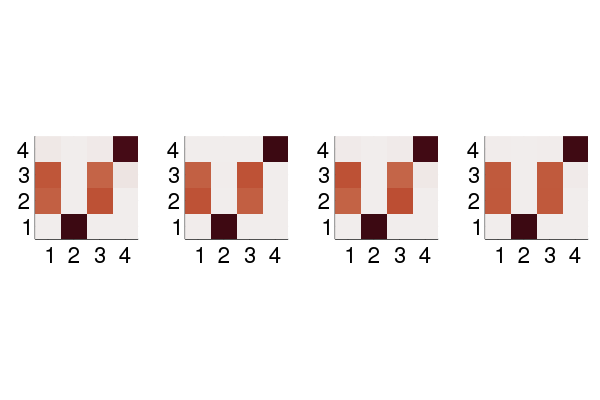
\includegraphics[width=0.9\linewidth]{swapmats}
% 	\caption{Analysis of Replica Exchange}
% 	\label{swapmats}
% \end{figure}	


\begin{figure}[!htb]
	\centering
	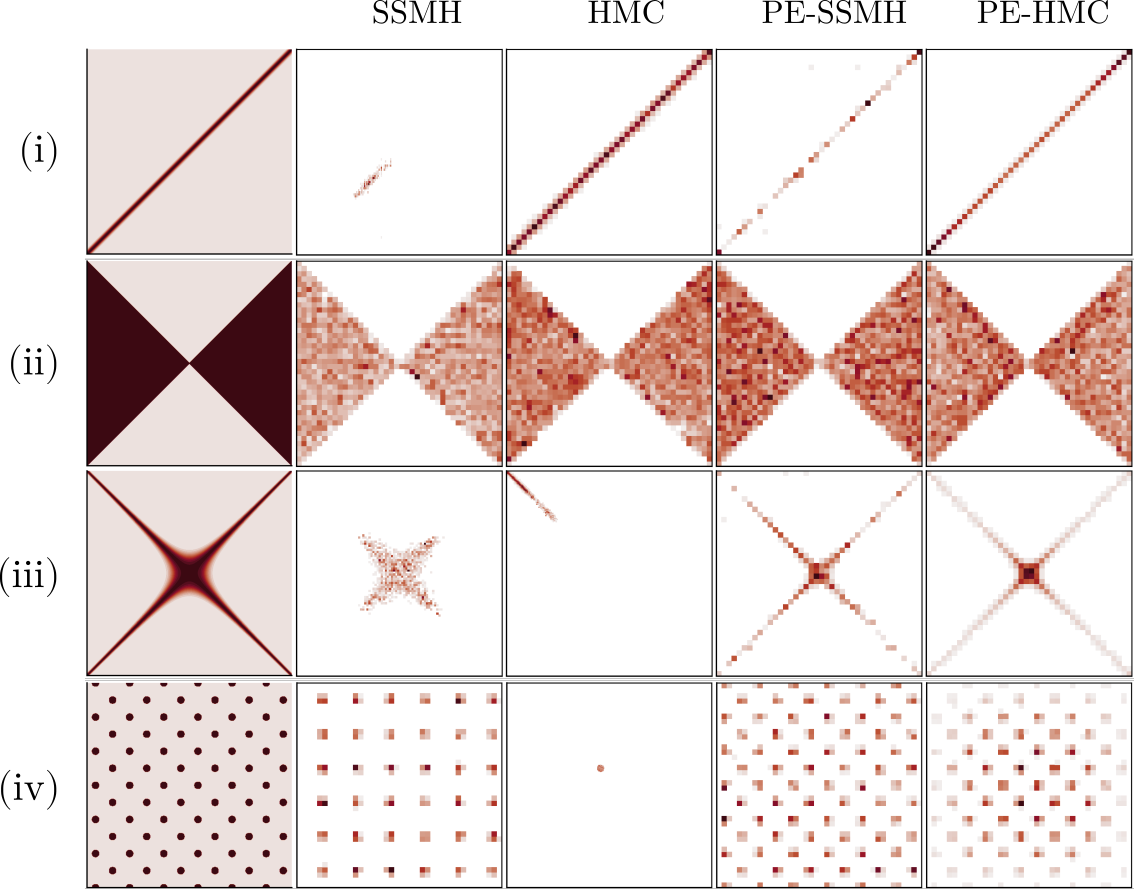
\includegraphics[width=0.9\linewidth]{gx2}
	\caption{Samples from models using different procedures.  Each model is $x,y \sim \unif(-1,1)$ conditioned on (i) $x \soft{=} y$, (ii) $|x| \soft{>} |y|$, (iii) $x^2 \soft{=} y^2$ and (iv) $\sin(kx)\cos(kx) \soft{>} 0.9999$.
	Inference procedures are: Single Site Metropolis Hastings (SSMH), Hamiltonian Monte Carlo (HMC), and Predicate-Exchange (PE) using HMC and SSMH within chain.}
	\label{gridn}
\end{figure}	

\begin{figure}[!htb]
\centering
\textbf{Truncated Normal through Conditioning}\par\medskip
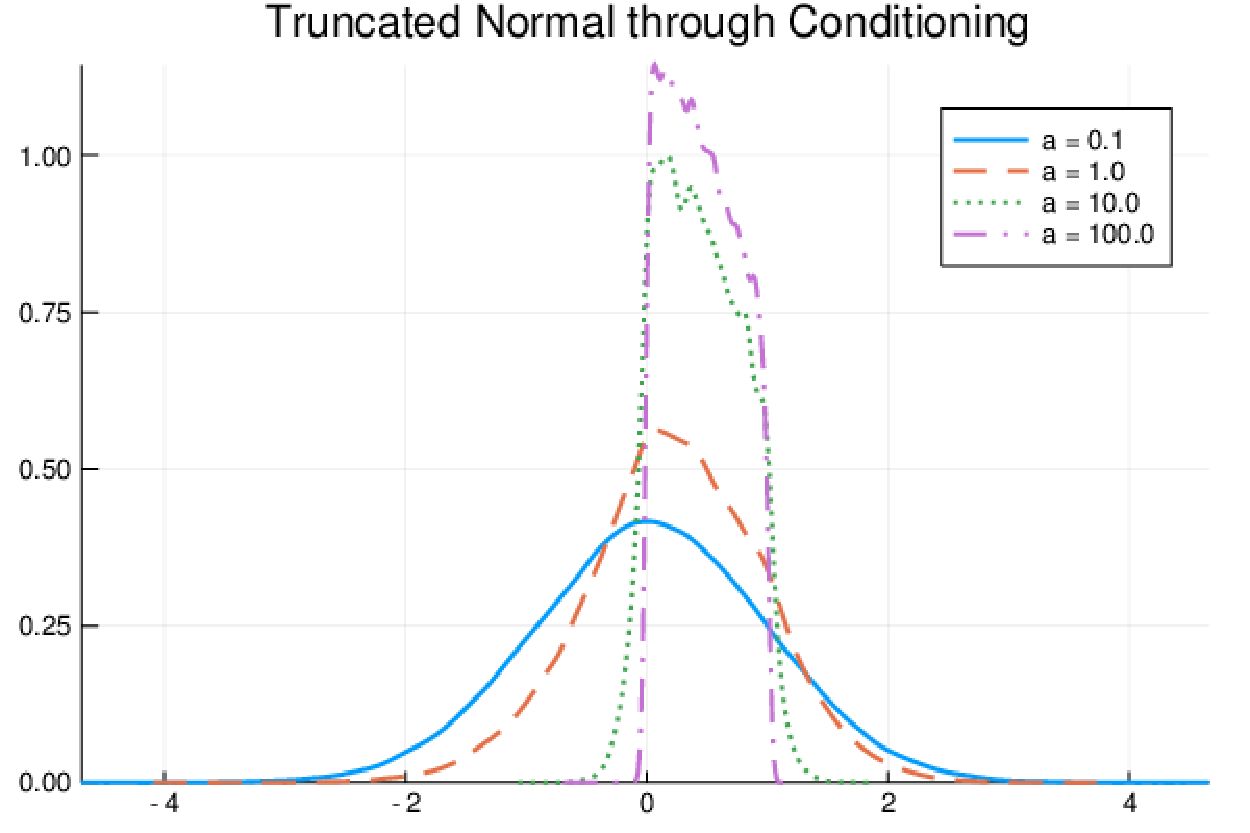
\includegraphics[width=0.55\linewidth,trim={0.5cm, .3cm, .5cm, .1cm}, clip]{truncated}
% \fbox{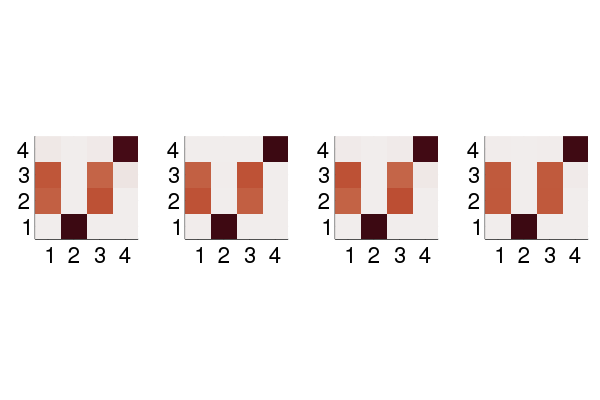
\includegraphics[width=0.40\linewidth,trim={2.0cm, .2cm, 2cm, 1.2cm}, clip]{swapmats}}
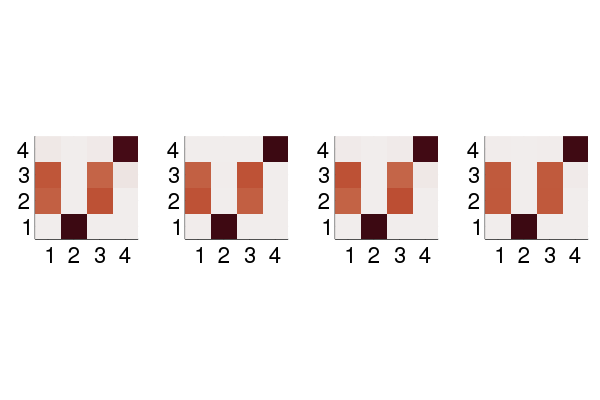
\includegraphics[width=0.40\linewidth,trim={2.0cm, .2cm, 2cm, 1.2cm}, clip]{swapmats}

% \fbox{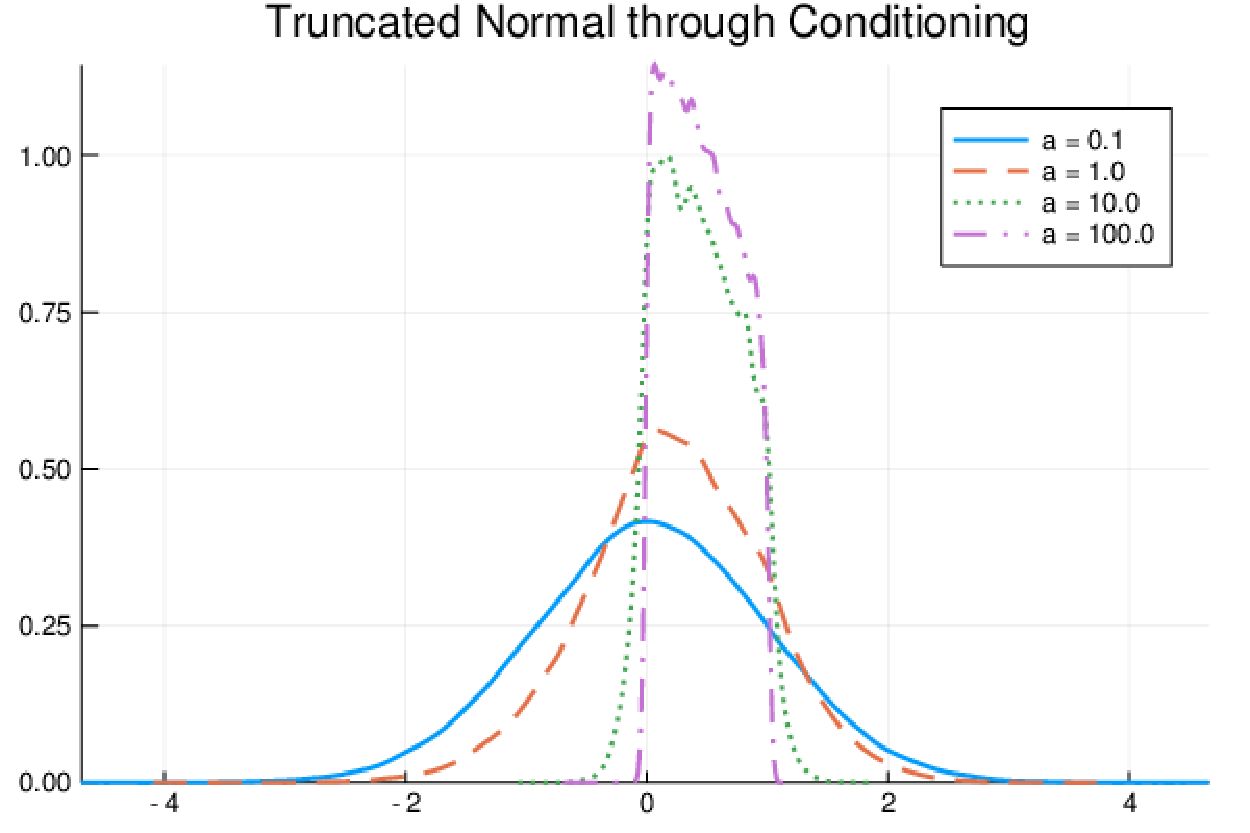
\includegraphics[width=1\linewidth,trim={0.5cm, .3cm, .5cm, .1cm}, clip]{truncated}}

% \begin{minipage}{0.45\linewidth}
% 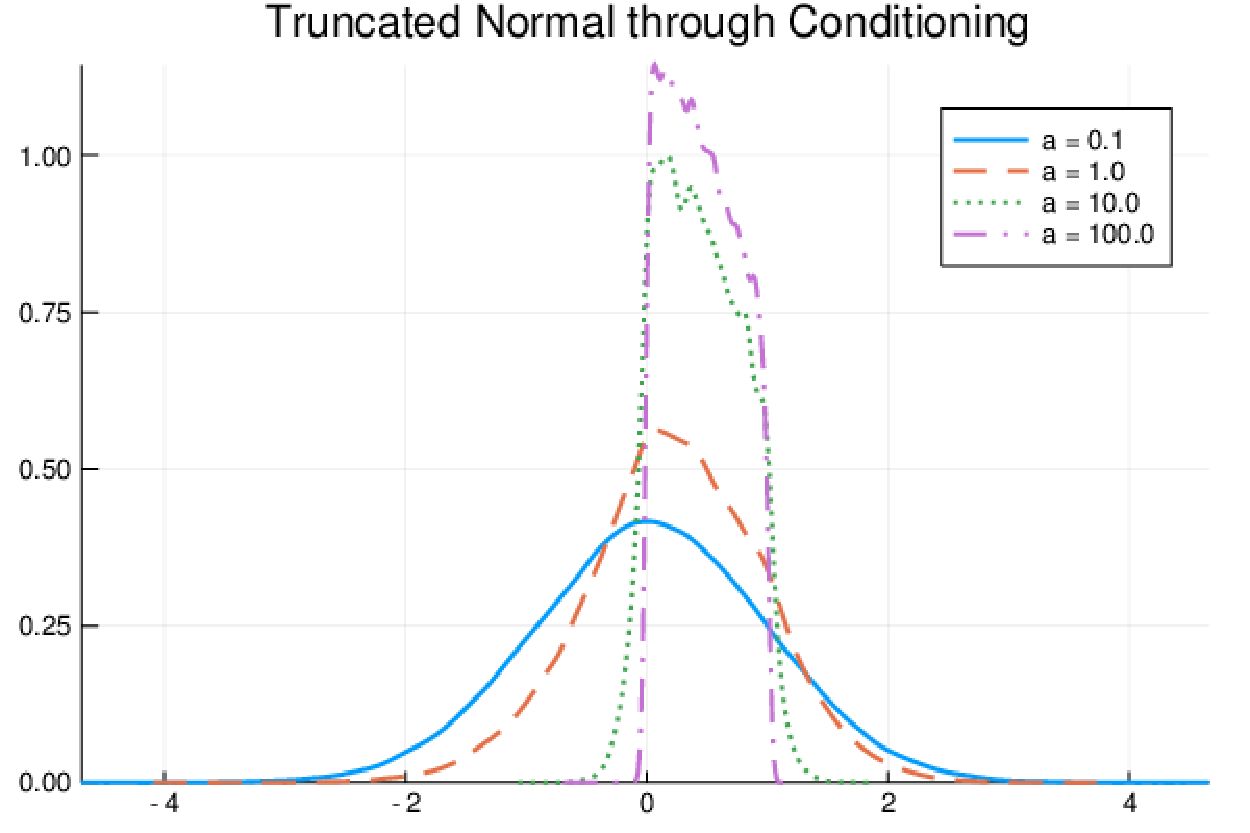
\includegraphics[width=\linewidth]{truncated}
% \end{minipage}%
% \begin{minipage}{0.45\linewidth}
% 	%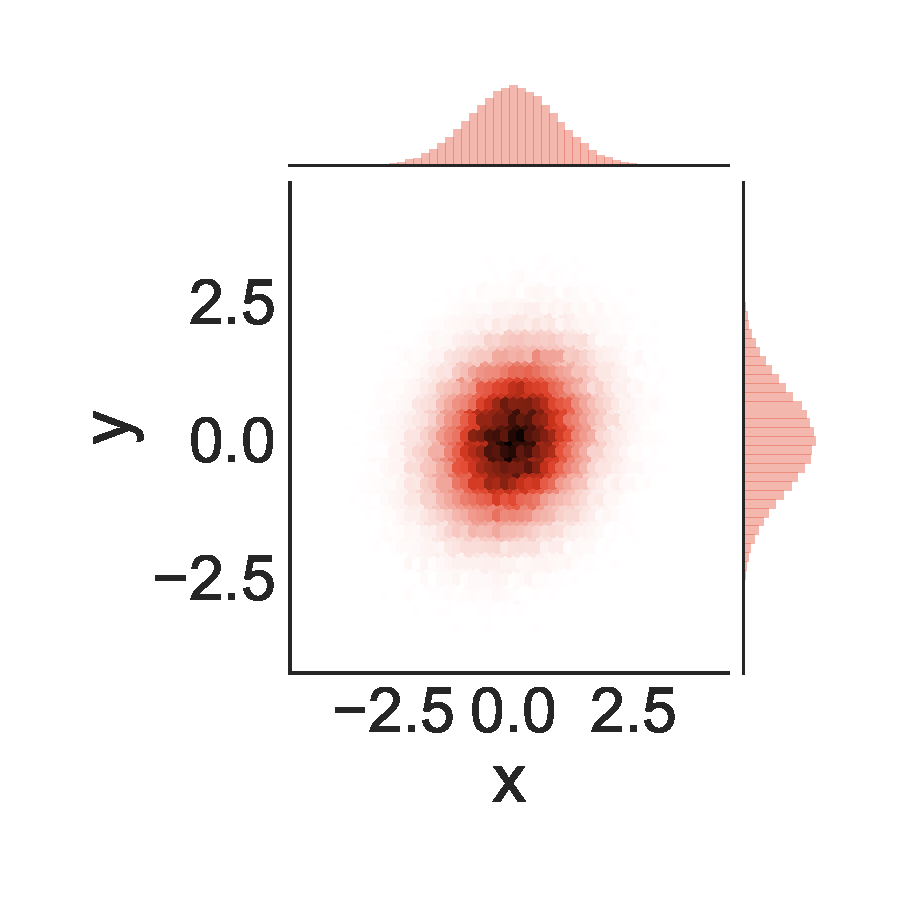
\includegraphics[width=.16\linewidth, trim={1.7cm, 1.6cm, 1.3cm, 1.5cm}, clip]{0-1}
% 	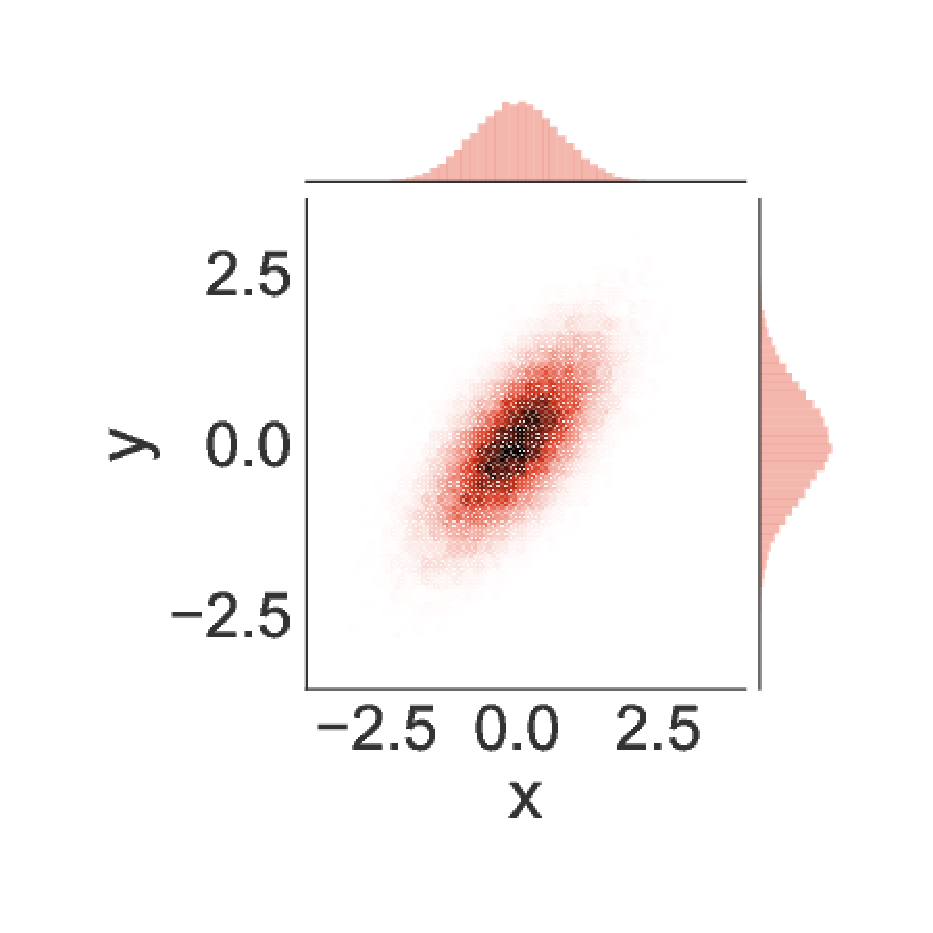
\includegraphics[width=.45\linewidth, trim={1.7cm, 1.6cm, 1.3cm, 1.5cm}, clip]{1-0}
% 	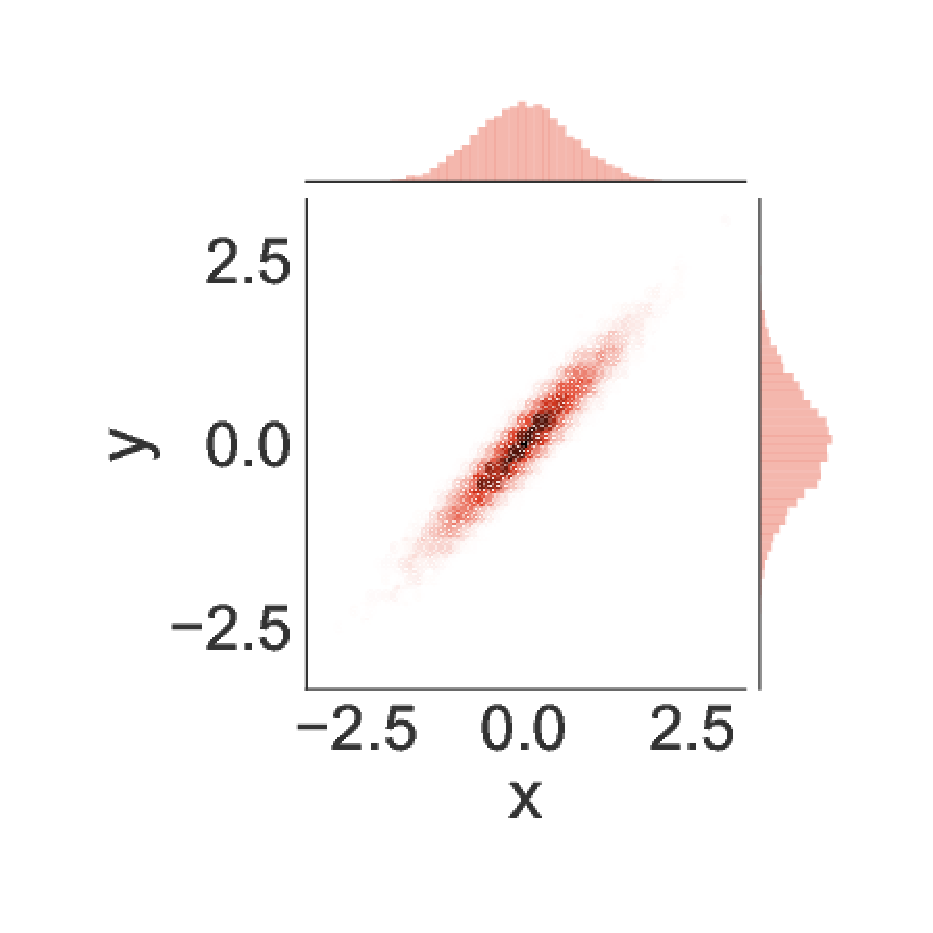
\includegraphics[width=.45\linewidth, trim={1.7cm, 1.6cm, 1.3cm, 1.5cm}, clip]{10-0}
	
% 	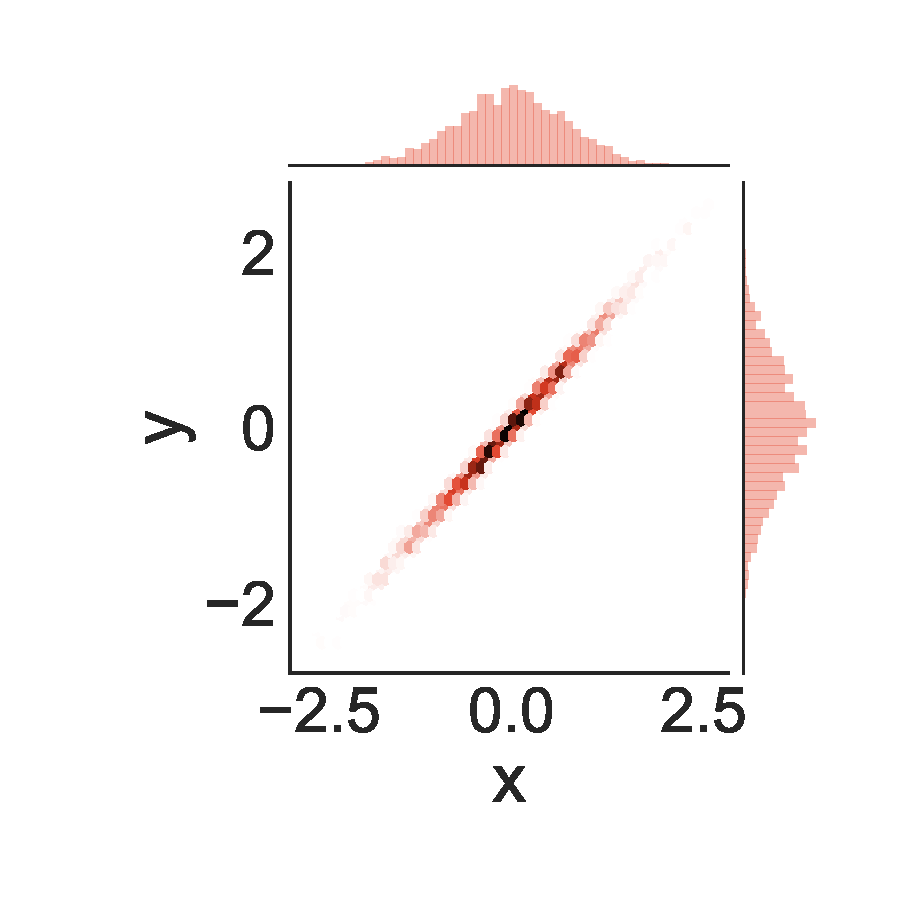
\includegraphics[width=.45\linewidth, trim={1.7cm, 1.6cm, 1.3cm, 1.5cm}, clip]{100-0}
% 	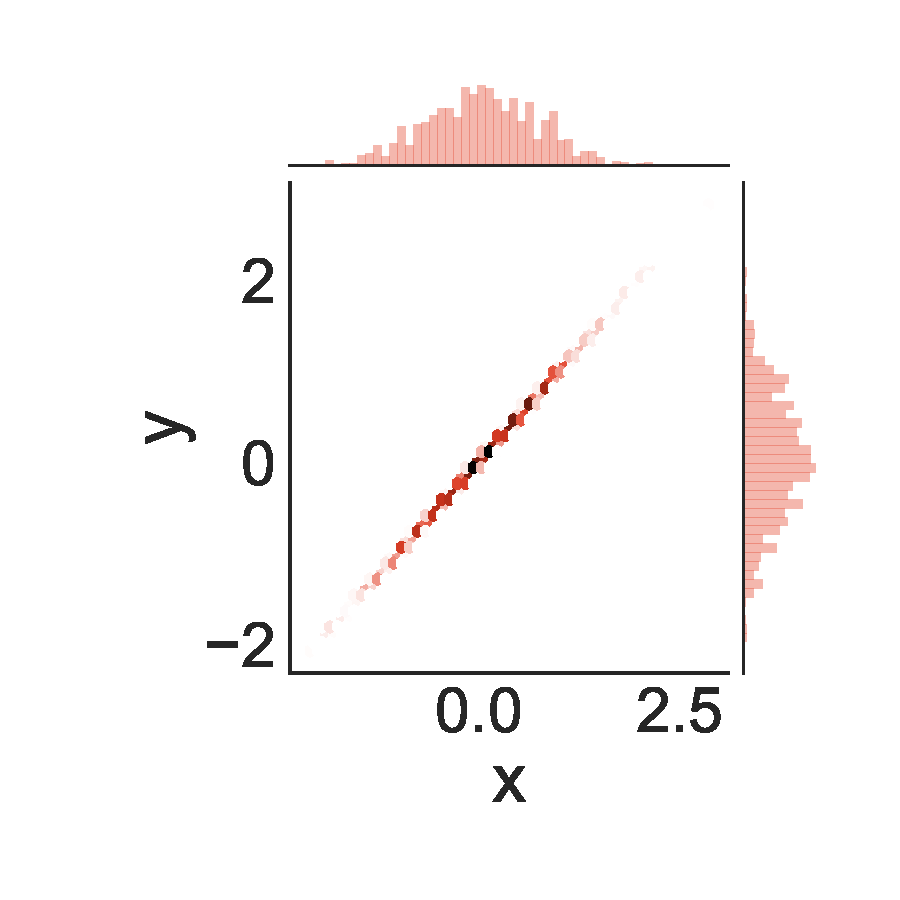
\includegraphics[width=.45\linewidth, trim={1.7cm, 1.6cm, 1.3cm, 1.5cm}, clip]{1000-0}				
	
% %	\fbox{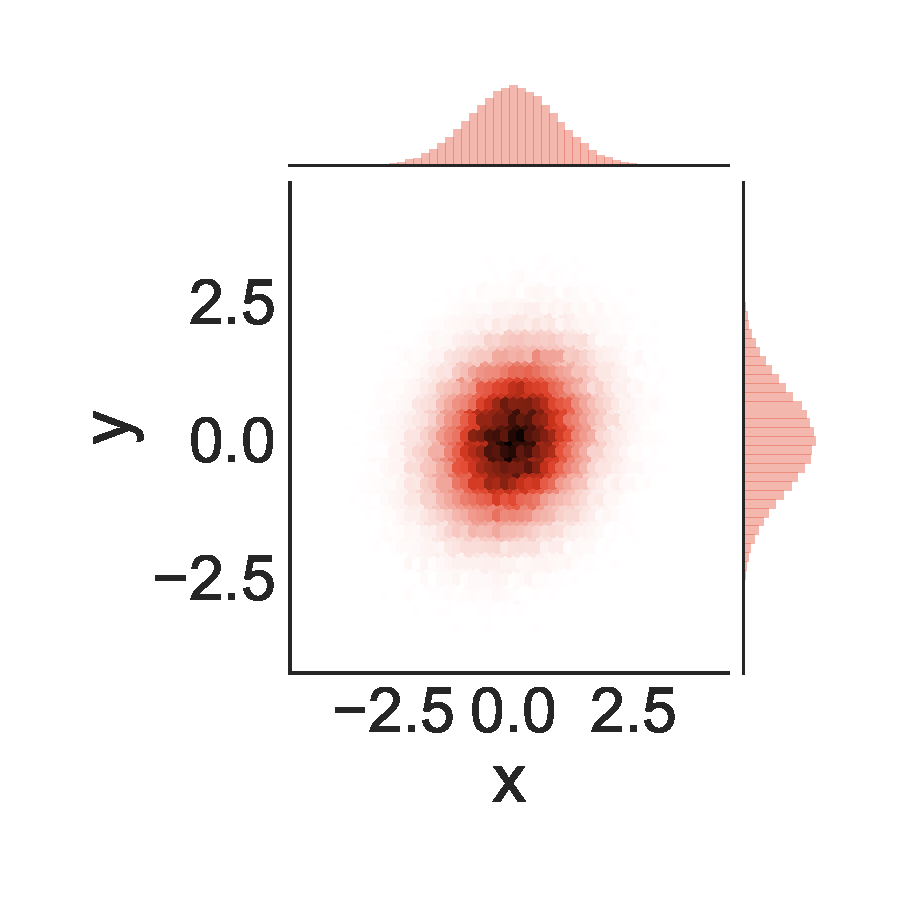
\includegraphics[width=.16\linewidth, trim={1.7cm, 1.6cm, 1.3cm, 1.5cm}, clip]{0-1}}
% %	\fbox{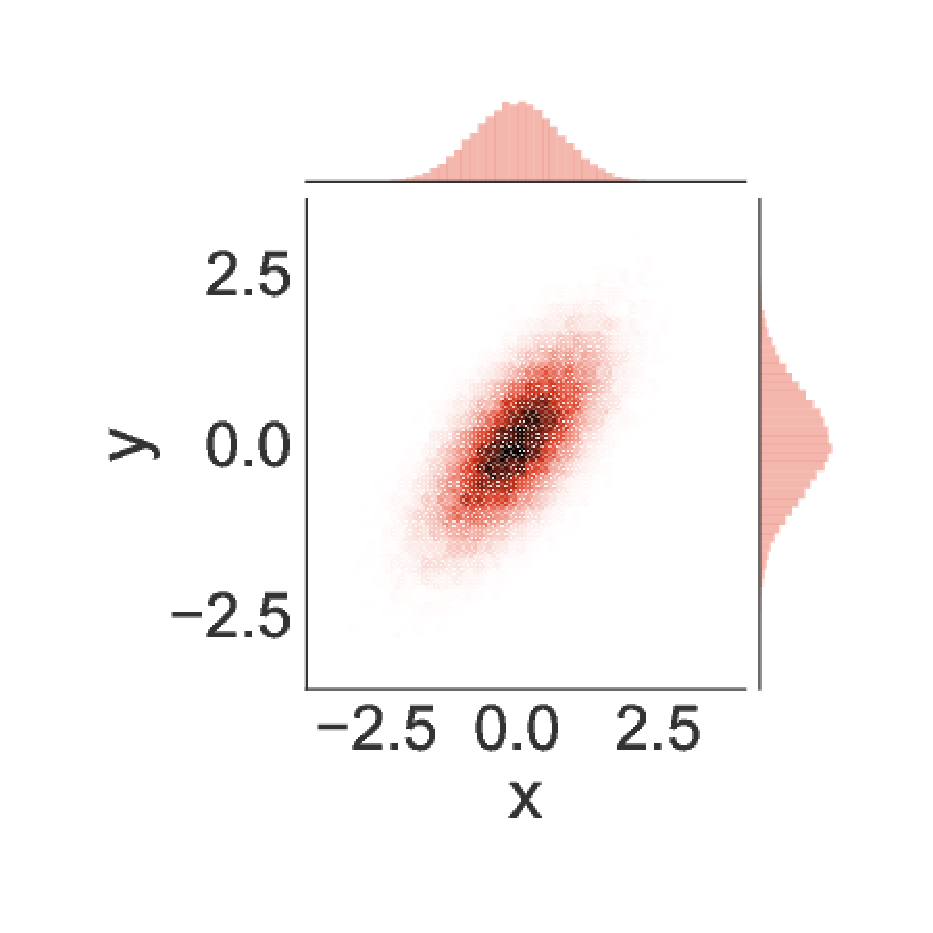
\includegraphics[width=.16\linewidth, trim={1.7cm, 1.6cm, 1.3cm, 1.5cm}, clip]{1-0}}
% %	\fbox{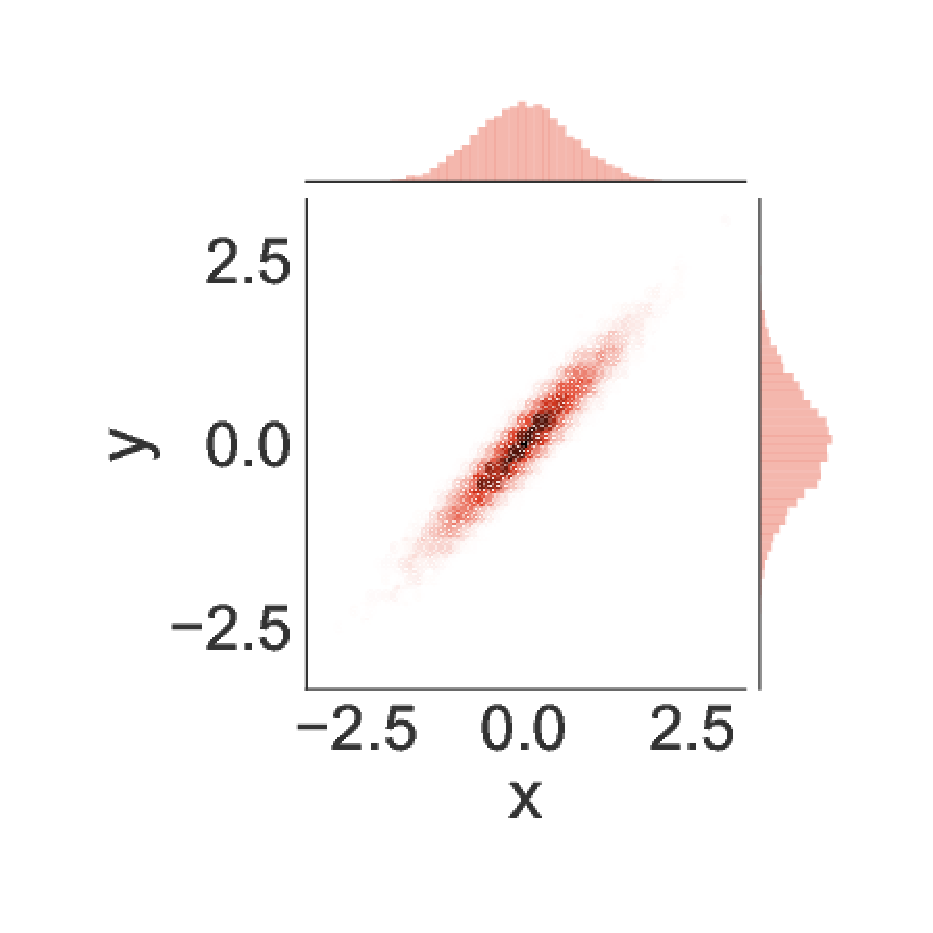
\includegraphics[width=.16\linewidth, trim={1.7cm, 1.6cm, 1.3cm, 1.5cm}, clip]{10-0}}
% %	\fbox{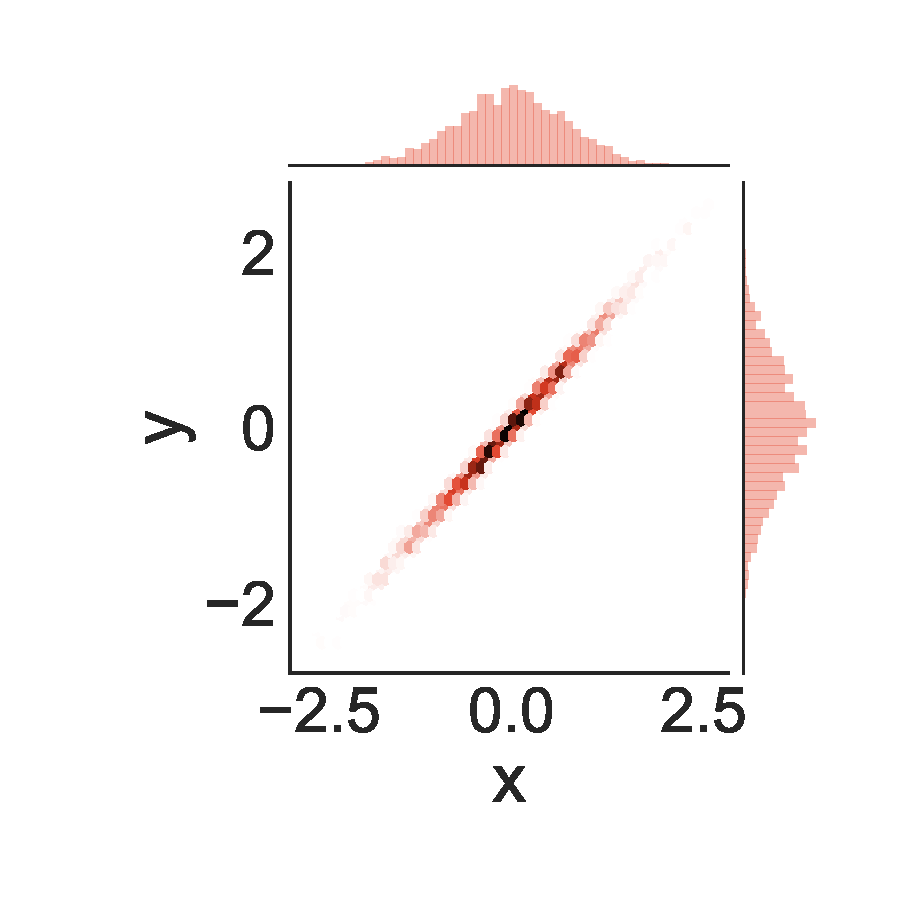
\includegraphics[width=.16\linewidth, trim={1.7cm, 1.6cm, 1.3cm, 1.5cm}, clip]{100-0}}
% %	\fbox{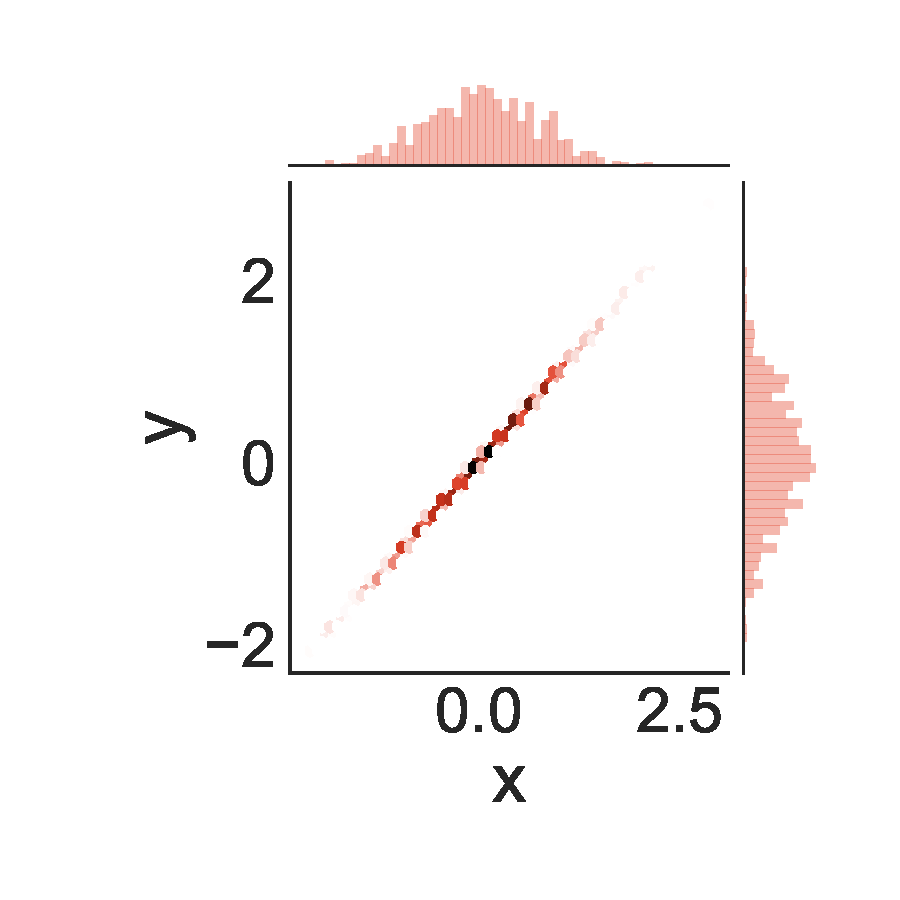
\includegraphics[width=.16\linewidth, trim={1.7cm, 1.6cm, 1.3cm, 1.5cm}, clip]{1000-0}}				
% 	\end{minipage}
	\caption{Kernel density estimation from samples of Gaussian truncated to $[0, 1]$ through conditioning. Shown at different temperatures.}
	\label{fig:density}
\end{figure}



\paragraph{Inverse Ray Tracing}
In this example we sample from a posterior distribution over scenes conditioned an observed rendering.  A scene $s$ is a set of $n \sim \textrm{poisson}(\lambda = 3)$ spheres.
A sphere is parameterized by color, reflectance, emission color, transparency, radius and position, all with a uniform prior.
Let $r$ be a ray tracing function that maps scenes to image, $i_{obs}$ be an observed image, and $\textrm{nointersect}$ be a predicate that maps a scene to 1 iff any spheres intersect.
The prior $s$ is conditioned on the conjunction of the inverse rendering and the no-intersection constraints:

\begin{equation}
(r(s) = i_{obs}) \land \textrm{nointersect}(s)
\end{equation}

Figure \ref{fig:invrtmcmc} visualizes conditional samples.
% \begin{figure}
% 	\centering
% 	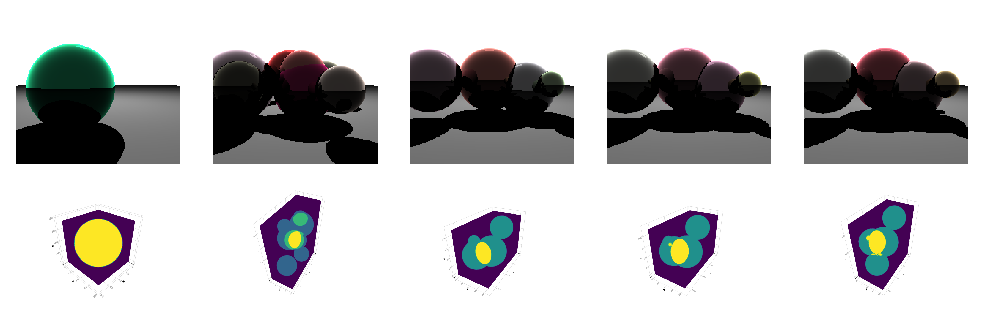
\includegraphics[width=0.9\linewidth]{invg2.pdf}
% 	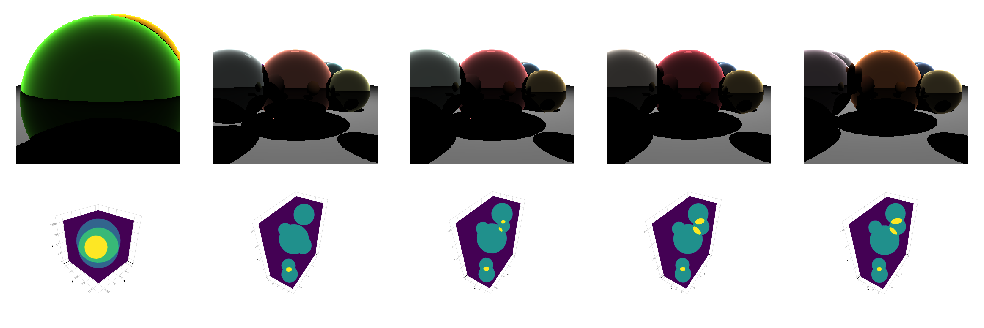
\includegraphics[width=0.9\linewidth]{invgb.pdf}
% 	% 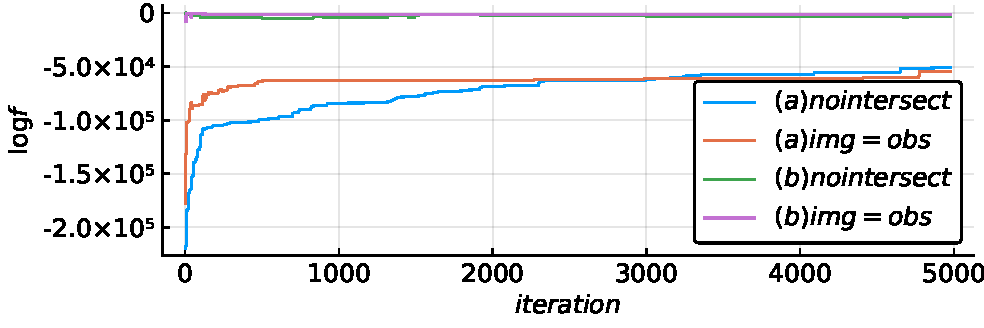
\includegraphics[width=0.9\linewidth]{lvstime.pdf}
% 	% 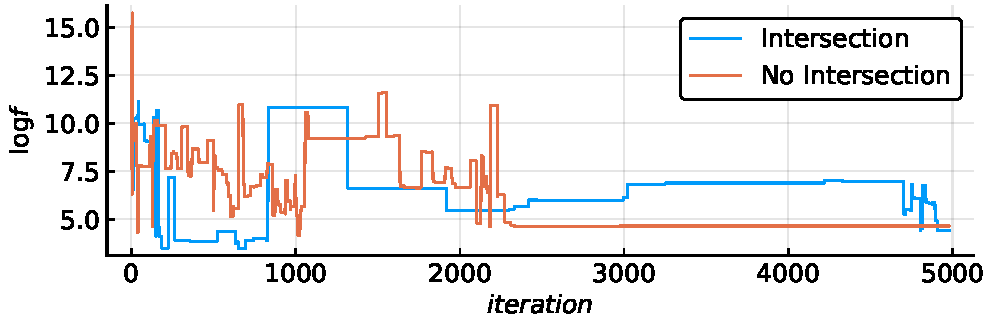
\includegraphics[width=0.9\linewidth]{Hausdorf.pdf}
% 	\caption{ Samples from inverse graphics.}
% 	\label{fig:invrtmcmc}
% \end{figure}

\begin{figure}
	\centering
	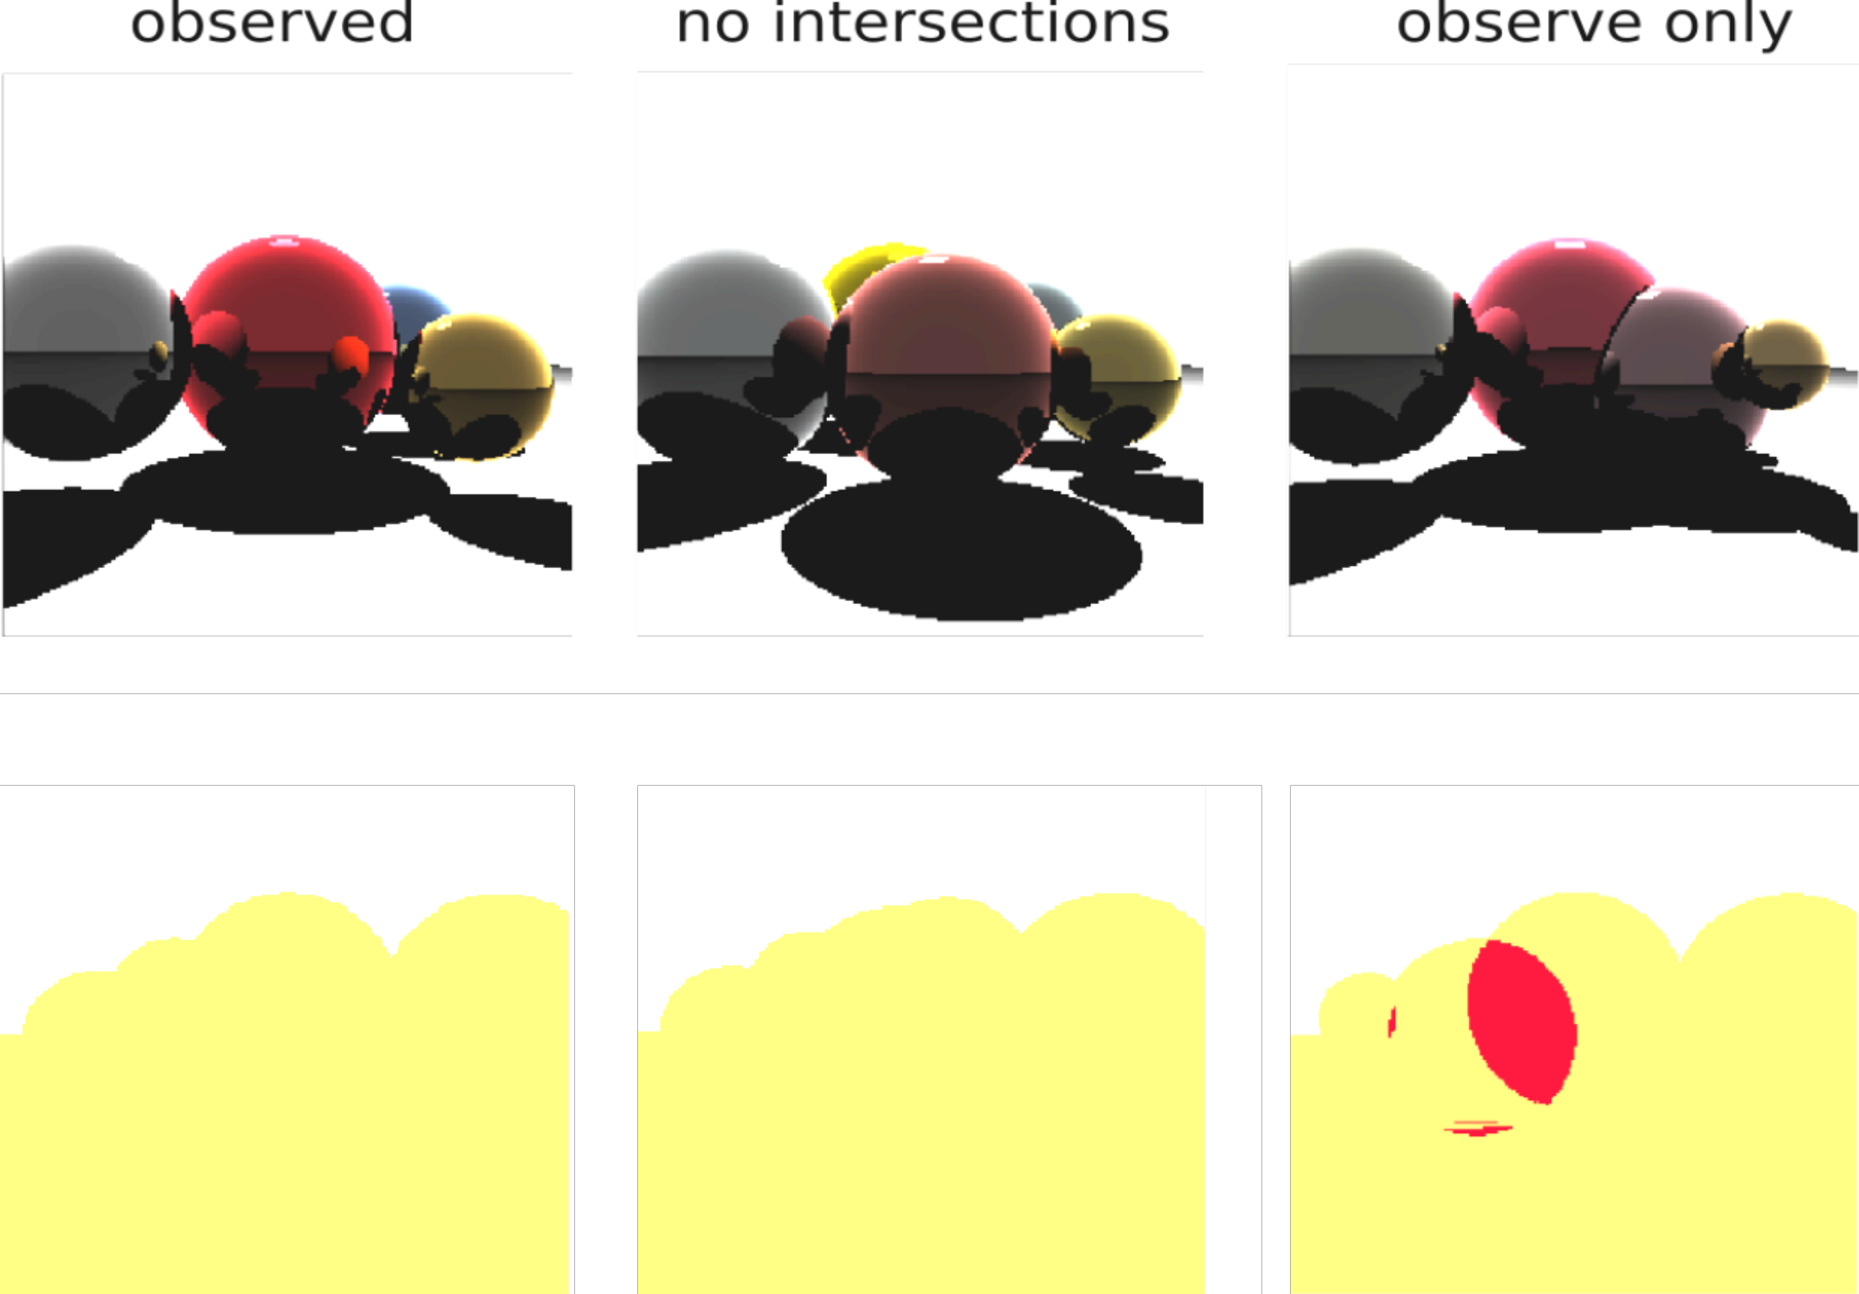
\includegraphics[width=0.9\linewidth]{jampy2.pdf}
	\caption{Inverse rendering with and without no-intersection constraints.  Top row: raytraced scenes.  Bottom row: red pixels denote the existence of an intersection between spheres at that point.  (middle) and (right) scenes are samples from posterior over scenes having observed image on left.  The observed scene has no intersections.  Without the no-intersection condition (right), intersections occur.  Conditioning on intersection eliminates intersections (middle).}
	\label{fig:invrtmcmc}
\end{figure}


\paragraph{Glucose Model}
Type 2 diabetes is a prevalent and costly condition.
Keeping blood glucose within normal limits helps prevent the
long-term complications of Type 2 diabetes like diabetic neuropathy and diabetic retinopathy \citep{brownlee2006glycemic}. Models to predict the trajectories of blood glucose aid in keeping glucose within
normal limits \citep{zeevi2015personalized}. Traditional models have been built from compositions of differential equations \citep{albers2017personalized,levine2017offline} whose parameters are estimated separately for each patient. An alternative approach would be to use a flexible sequence model like an RNN. The problem with this approach is that an RNN can extrapolate to glucose values incompatible with human physiology. This is especially a problem where we have patients with only a few blood glucose measurements. To build an RNN model that respects physiology, we condition on it.

We compare the independent RNN model to the one with declarative knowledge on a second patient from Physionet \citep{moody2001physionet}.
Figure \ref{fig:rnn-samples} plots the results performed on more than 300 pairs of patients.
We see that the conditional model simulates
more realistic glucose dynamics for the patient 
with only a short observed time-series.

% 1) Glucose modeling is a real problem \cite, \cite. 
% 2) Models have focused on ODEs \cite \cite 
% 3) Alternative is to use RNN 
% 4) RNN can produce nonsense result 
% 5) Conditioning helps


% Taken from the supplement in \cite{albers}

% \paragraph{A constrained model of glucose dynamic}
% Take glucose measurements across time $t$ from 
% N patients indexed by $i$: $x_{t,i}$.
% We model the glucose time series for each patient can be modeled independently using a recurrent neural network: 
% \begin{align*}
% W_i &\sim N(0, I) \\
% x_{t, i} &= f(x_{t-1, i}, W).
% \end{align*}
% This model treats all patients as independent. However,
% we have extra knowledge in that the average-across-time glucose levels will be similar across patients. Expressing this kind of knowledge by tying the parameters $W_i, W_j$ is a challenge because the structure of the recurrence function alters how $W$ controls the average outputs. In this sense, we would like to condition on the distance between conditional expectations being close for some distance $d$,
% \begin{align*}
% 	E\left(\sum_{t=1}^{T_i} E[x_{t, i} \,|\, W_i], \sum_{t=1}^{T_j} E[x_{t, j} \,|\, W_j]\right) < \delta_E,
% \end{align*}
% for all patient pairs $i, j$. Additionally, we would like to make the series smooth controlling for their variance:
% \begin{align*}
% 	d_{Var}\left(\sum_{t=1}^{T_i} Var[x_{t, i} \,|\, W_i], \sum_{t=1}^{T_j} Var[x_{t, j} \,|\, W_j]\right) < \delta_{Var},
% \end{align*}
%  We compare the independent model
% to the one with the conditional model learned on five patients. 
% We see that the conditional model simulates more realistic glucose dynamics for the patient with only a short observed time-series.

\begin{figure}[!htb]
	\centering
    %\fbox{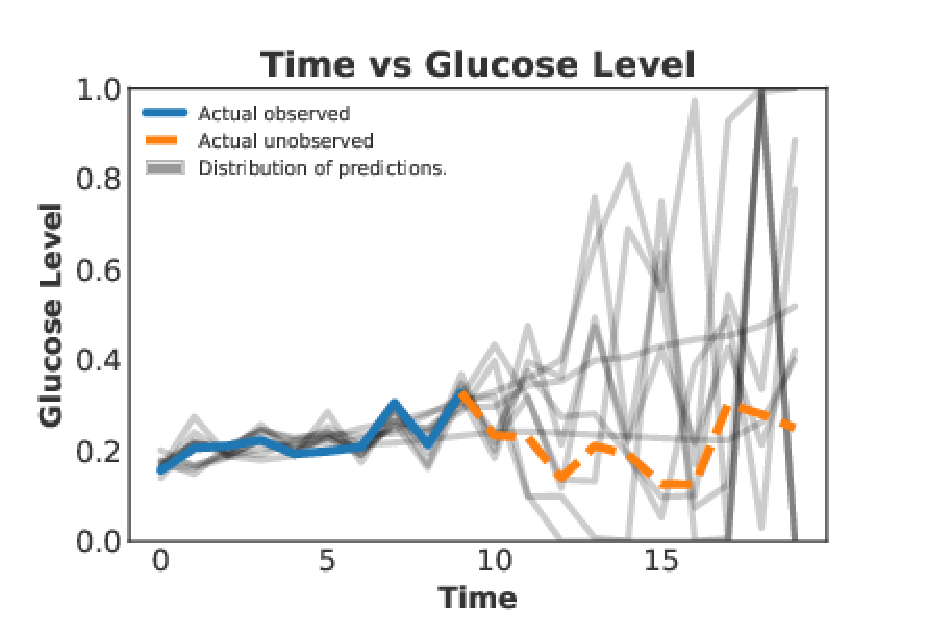
\includegraphics[width=0.30\linewidth, trim={1.cm, 0.1cm, 1.3cm, .5cm}, clip]{rnnsamples-no-tie-py}}
	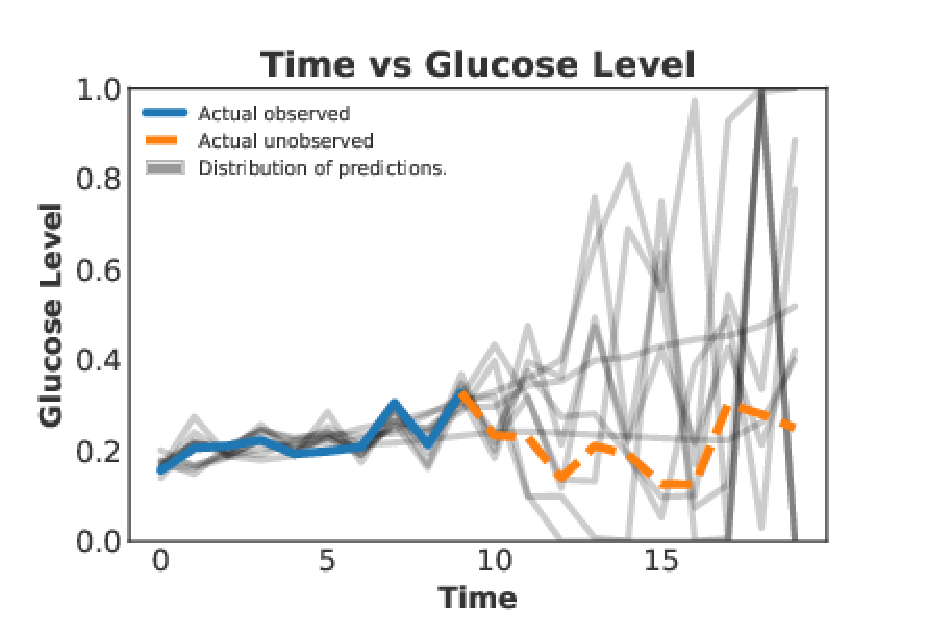
\includegraphics[width=0.8\linewidth, trim={1.cm, 0.1cm, 1.3cm, .5cm}, clip]{rnnsamples-no-tie-py}
	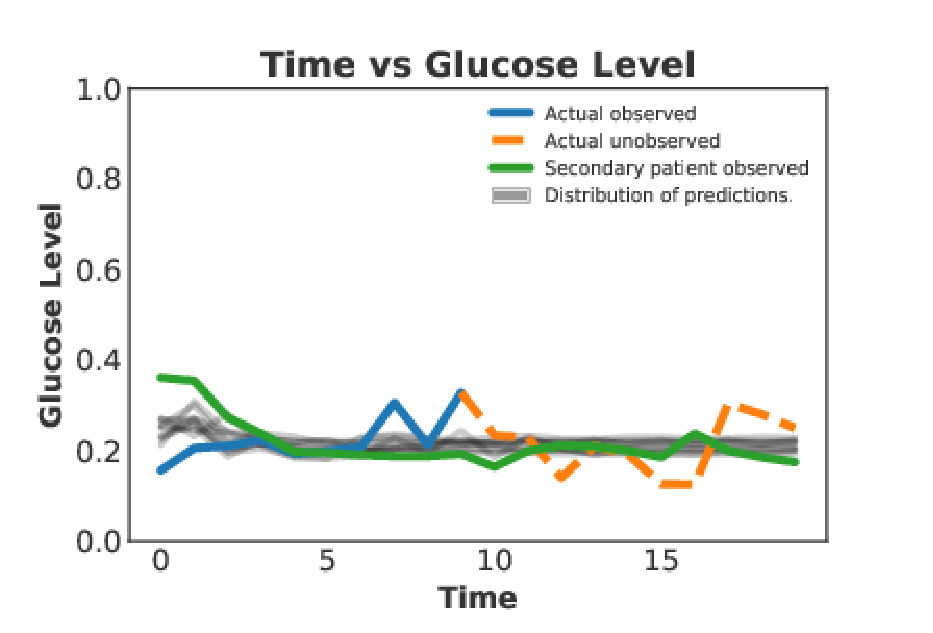
\includegraphics[width=0.8\linewidth, trim={1.cm, 0.1cm, 1.3cm, .5cm}, clip]{rnnsamples-py}
	%\fbox{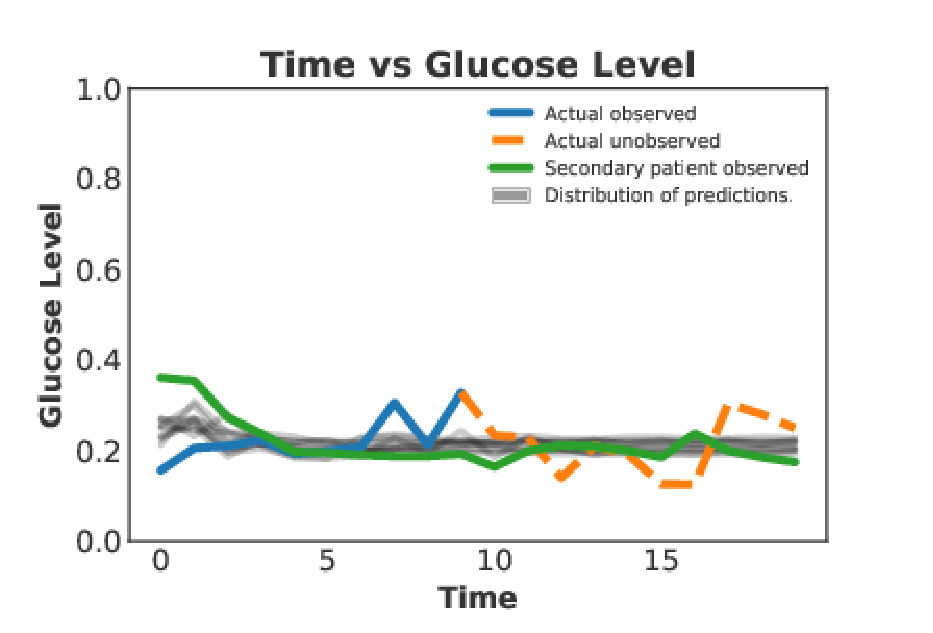
\includegraphics[width=0.30\linewidth, trim={1.cm, 0.1cm, 1.3cm, .5cm}, clip]{rnnsamples-py}}
	%\fbox{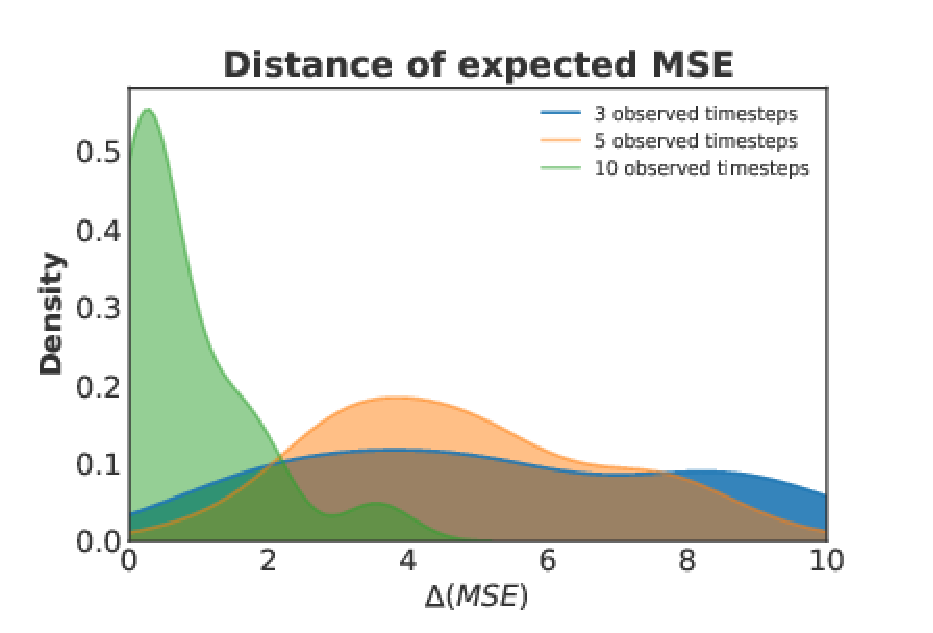
\includegraphics[width=0.30\linewidth, trim={1.cm, 0.0cm, 1.0cm, .5cm}, clip]{delta_mse}}
	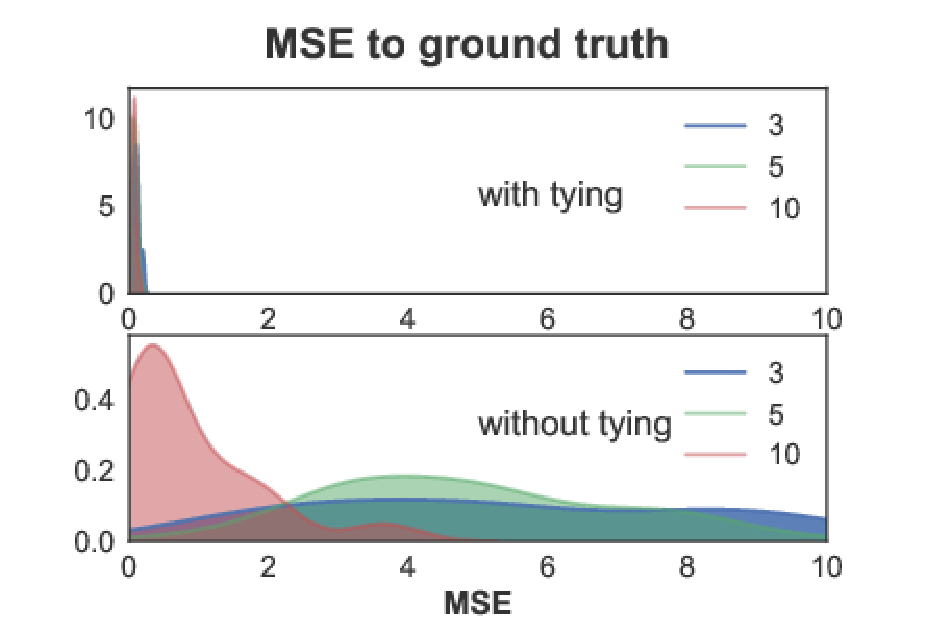
\includegraphics[width=0.9\linewidth, trim={0.7cm, 0.0cm, .7cm, .1cm}, clip]{mse}
		
		\caption{Left: Actual (dotted) and predicted trajectories that were learned using a partial trajectory. Center: Distribution of predicted trajectories learned only using the first ten data points and a tie with a secondary patient. Right, top: MSE when tie is present.  Right, bottom: without tie.  Tying expectations has dramatic influence on prediction error, while as more data is observed, the effect of tying decreases.}
		\label{fig:rnn-samples}
\end{figure}



% Take the same glucose measurements from 5 patients. Make a probabilistic RNN with
% independent parameters for each patient. Then add the constraint that the means are
% close. Then look at the prediction for one patient where we remove all but the
% first few time steps and show the forward predictions are better with the added knowledge
% that the means are close across patients.


% \paragraph{Transfer Learning}
% In transfer learning, we hope to use information from one learning problem to
% help with another learning problem. One way this has been accomplished in
% deep learning is to use
% the parameters of a model learned in one domain as the initialization for the
% parameters in a another domain. We could accomplish a similar thing via conditioning
% by having the weights of both models be close. But with conditioning, this is not
% the only choice, we can have the first layer activations be close in distribution
% in both the source and target transfer domain. Concretely, consider the following
% two layer stochastic neural network for each domain where the $i$th covariate
% label pair $(x_i, y_i)$ is
% \begin{align*}
% W \sim p(W)
% z_{2, i} &\sim p(z_{2, i} | x_i, W_2) \\
% z_{1, i} &\sim p(z_{1, i} | z_{2, i}, W_1) \\
% y_{i} &\sim p(y_i | z_{1, i})
% \end{align*}


% \section{Related Work}
% \begin{itemize}

% \item Existing Notion of Probablistic Programs
% Probabilistic programming languages and the inference algorithms which support them differ primarily in how probability distributions are represented.
% % In this contribution we define the sample space as an $n$-dimensional unit hypercube
% % $\Omega = [0, 1]^n$, and by $(\omega_1,...,\omega_n)$ denote an element of $\Omega$.
% % In addition, we define $\mu$ as the Lebesgue measure.
% % Random variables are transformations of $\Omega$, and act on some or all of its dimensions.
% % For example a random variable $\mathcal{U}_{a,b}: \Omega \to \mathbb{R}$, which is distributed uniformly between $a$ and $b$ could be defined simply as:
% % $$
% % \mathcal{U}_{a,b}(\omega) = a + \omega_1(b - a)
% % $$
% \item Make explicit how the measure theortic formulation connects to the sampling process
% \end{itemize}


\paragraph{Benchmarks}
To quantitatively compare predicate exchange with existing approaches we constructed an artificial problem that scales in difficulty.
Let $X_i \sim \mathcal{N}(0,1)$ in a $d$-dimensional model $\vect{X} = (X_1, \dots, X_d)$ conditioned on an $\epsilon$-thick ring:
\begin{equation}
\lk_\epsilon(\vect{x}) = 1 < |\vect{x}| < 1 + \epsilon
\end{equation}

Table \ref{results} compares the sample average of particle Gibbs (PG), sequential Monte Carlo (SMC), rejection sampling (RS) and predicate exchange (PE), varying both $\epsilon$ and $d$.
The theoretical expectation of all models is 0.
Among these methods, predicate exchange is unique in its support for inference with predicates, which makes direct comparison difficult.
For all inference procedures we use predicate relaxation to compute $d = \softv{\lk}_\epsilon(\vect{x})$, and sample from $\vect{X}$ conditioned on $\mathcal{N}(d, 1/(2\alpha)) = 1$, where $\alpha$ is the lowest temperature used in predicate exchange.
Predicate exchange  compares favourably in most scenarios.


\begin{figure}
\begin{center}
	\begin{tabular}{||c| c c c c||} 
	\hline
	 $d,\epsilon$& $1, {10^{-1}}$ & $1, {10^{-5}}$ & ${100}, {10^{-1}}$ & ${100}, {10^{-5}}$ \\ [0.5ex] 
	\hline\hline
	PE & 0.0054 & 0.4735  & -0.00037 & 0.00854\\ 
	\hline
	% HMC & 2.1 & 2.026  & 1.5 & 1.41\\ 
	% \hline\hline
	SMC & 0.06 & -0.226  & -0.018 & 0.09\\ 
	\hline
	PG & -0.029 & 0.239 & -0.03 & 0.03\\
	\hline
	RS & 0.003 & timeout & timeout & timeout \\
	\hline
 \end{tabular}
 \label{results}
 \caption{Comparison of expectations of samples from $d$ dimensional ring.  Theoretical value is 0 in all cases.}
 \end{center}
\end{figure}


  
\section{Related Work}

% Likelihood free inference
Demand for likelihood-free inference emerged in genetics ecology.
Tavar{\'e} et al. \yrcite{tavare1997inferring} 
filtered samples from a stochastic simulator to only those which matched (according to summary statistics) observed data. 
%  to perform one of the earliest forms of likelihood-free inference.
Weiss et al. \yrcite{weiss1998inference} extended this with a tolerance term, so that simulations sufficiently close to the data were accepted.
% Such posterior samples are therefore approximate.
A variety of approaches in this general regime  \cite{beaumont2002approximate,sisson2007sequential} fall under the heading of Approximate Bayesian Computation (ABC).
Marjoram et al. \yrcite{marjoram2003markov} simulated Markov Chains according to the prior, but applied the same summary statistic based filtering to yield approximate posterior samples.
A small tolerance leads to a high rate of rejected simulations, whereas a large tolerance results in an unacceptable approximation error.
Among several solutions are dynamically decreasing the tolerance \cite{toni2008approximate}, importance reweighting samples based on distance \cite{wegmann2009efficient}, adapting the tolerance based on distance \cite{del2012adaptive,lenormand2013adaptive}, as well as annealing the tolerance as a temperature parameter \cite{albert2015simulated}.

% Despite widespread use in physics, replica exchange  has seen only limited application to Bayesian inference problems.
% In a notable exception \cite{habeck2005replica} reparametrize both the prior and likelihood terms in the Bayesian posterior with two extra parameters, which independently control the influence of the likelihood function, and replace the prior
% $\pi(\theta)$ by $\pi(\theta; q) \propto \exp(-\beta E(\theta; q))$, where $E$  Tsallis generalization  
% Baragatti et al. \cite{baragatti2013likelihood} construct an parallel chains where the temperature of each chain is set at the tolerance parameter.


Predicate exchange targets simulation models and uses distance metrics, but performs asymptotically exact inference without summary statistics.
A recent approach \cite{graham2017asymptotically}  with similar objectives develops a Hamiltonian Monte Carlo variant, using a quasi-Newton method during leap-frog integration to exactly solve the observation constraint.
This is limited to differentiable models conditioned with equality.
Predicate exchange is not limited to differentiable models, but is approximate when the condition is of measure zero.

% PPLS
Probabilistic logics such as ProbLog \cite{richardson2006markov} and Markov logic networks \cite{de2007problog} extend first order logic to express both models and conditions.
Of particular note, probabilistic soft logic (PSL) \cite{brocheler2012probabilistic,kimmig2012short} uses continuous logic to encode graded beliefs.
For example, $\text{isfriend(Alice, Bob)} \to 0.9$ denotes a strong friendship between Alice and Bob.
The primary distinction between PSL and predicate exchange is in the semantics of the soft predicates.
In predicate exchange, relaxation is used solely to make inference more tractable; soft Boolean values are used only within the sampling process and do not appear in the resulting samples themselves.
In addition, predicate exchange is motivated by probabilistic programming languages for generative models, such as ~\citep{milch20071, wood2014new,mansinghka2014venture,goodman2008church}, rather than purely declarative logic based languages.


Several continuous \cite{levin2000continuous} and fuzzy \cite{klir1995fuzzy} logics apply model-theoretic tools to metric structures.
Continuous logics replace the Boolean structure $\{T, F\}$, quantifiers $\forall x$ and $\exists x$, and logical connectives with continuous counter-parts.
Predicate uses continuous logic to make inference more tractable. Semantically, our approach remains within measure theoretic foundations, which relies on hard predicates to condition.
% Talk about Soft logic




\section{Discussion}
In this work we expanded the class of predicates that probabilistic models can be conditioned on in practice.

Control flow remains a challenge, and is related to the path explosion problem in program analysis.
Various strategies have been developed \cite{cadar2008exe, sen2005cute} to mitigate this, largely for automated tested.
Future work is to explore the extent to which these concepts can be adapted to the probabilistic domain.

There are several inference strategies other than replica exchange MCMC that could exploit predicate relaxation.
Maximum posterior inference is the most immediate option, which would entail maximizing equation \ref{fpm}.

% Black-box inference methods have gained significant traction due to how general, flexible, a vs grey box

Our approach comes with certain limitations.
Equality conditions on continuous variables indicate sets of zero measure.
This is problematic because the probability of proposing a satisfying state in a Markov chain becomes zero.
In these cases predicate exchange must sample at a minimum temperature strictly greater than zero, which is approximate.
Another limitation occurs if a predicate has branches (e.g., if-then-else statements) such that the execution-path taken depends on uncertainty in the model.
Such branches make it more difficult to estimate how close values of variables are to satisfying a predicate.

% \section{mathkey (delete me, later)}

\begin{enumerate}
\item $X$ - arbitrary random variable
\item \item $\cM$ - a model
\item $Y$ - Predicate to condition on
\item $\softv{Y}$ - Relaxation of $Y$ 
\item $f$ - posterior density
\item $p$ - prior density
\item $\lk$ - approximate likelihood (mistake there)
\item $\soft{\textrm{op}}$ - Relaxation of predicate $\textrm{op}$
\item $\cond$ - Operator in simulation model for conditioning
\item $\softv{y}$ - Soft Boolean element, i.e. in $[0, 1]$
\item $\pi$ - Simulation program
\item $\mathbb{D}$ dictionary
\item $k_\alpha$ - relxation kernel, parameterized by $\alpha$
\end{enumerate}


\bibliography{bib}
\bibliographystyle{icml2019}

\end{document}
